\documentclass[a4paper,12pt]{report}

\usepackage[italian]{babel}
\usepackage{hyperref}
\usepackage[utf8]{inputenc}
\usepackage{float}
\usepackage[table,xcdraw]{xcolor}
\usepackage{longtable}
\usepackage{graphicx}
\usepackage{todonotes}

\title{\textbf{CineRadar}\\Progetto di Basi di dati\\\textit{Università di Bologna}}
\author{Martin Tomassi; 0001077737\\Francesco Pazzaglia; 0001077423\\Luca Casadei; 0001069237}
\date{\today}

\begin{document}
\maketitle
\tableofcontents
\chapter{Analisi dei requisiti}
\section{Introduzione}
Il progetto consiste nella realizzazione di un applicativo per la condivisione e la recensione di elementi multimediali quali film e serie TV.
\section{Intervista}
È richiesto un sistema che consenta all'utenza di accedere al portale di condivisione di film e serie TV e poter recensirne uno o più di interesse, nel dettaglio, un film è un elemento multimediale unico, mentre una serie TV è composta da più stagioni, composte a loro volta da un certo numero di episodi. È necessario che l'utente si registri inserendo i propri dati che verranno salvaguardati, tra cui username, password, nome, cognome, data di nascita per controllare i limiti di età sui film. Un utente deve avere la possibilità di aggiungere nuovi film o serie nel sistema, ma non in maniera diretta, la richiesta deve prima essere approvata da un altro tipo di utente con privilegi di amministratore del sistema. L'amministratore si occuperà di aggiungere film alla piattaforma con frequenza settimanale. Sulle recensioni di altri utenti, un utente può esprimere un parere di utilità che andrà a classificare la recensione in una sorta di "classifica delle recensioni più utili". Quando si va a memorizzare un film o una serie TV bisogna inserire il titolo, uno o più autori, la descrizione, la durata, l'anno di rilascio ed eventuale casa produttrice. Gli utenti devono essere in grado di vedere tutti gli elementi multimediali presenti in base a dei filtri sul genere, categoria, autori e recensioni, sempre a patto che i risultati ottenuti rispettino i limiti di età standard dei film/serie (\textit{over 18, over 16} etc\dots). Quando un utente vede un film della lista, deve poterlo segnare come \textit{"già visto"} per poi poterlo recensire se lo desidera, mentre una stagione di una serie TV è considerata "vista" se tutti i suoi episodi sono stati contrassegnati come visti. Dato che si vogliono anche incentivare le famiglie, è richiesta una funzionalità che renda possibile inserire un'età e visualizzare i film/serie la cui visione è consentita (per esempio per capire se un film/serie è adatto per il proprio figlio). Un utente registrato all'interno dell'applicativo può ricevere, in base alla quantità e qualità delle sue recensioni, dei coupon da utilizzare all'interno di un cinema che ha erogato tale sconto, dopo aver ottenuto la loro tessera da affiliato. Il coupon può essere utilizzato per un elemento multimediale o genere specifico entro la sua data di scadenza. Sarà compito dei cinema stabilire quale impiegato avrà la facoltà di erogare le tessere. Per tenere traccia delle strutture che hanno emesso delle tessere vengono memorizzati i cinema attraverso un codice numerico, un indirizzo ed un nome. All'interno di ogni cinema è presente uno o più addetti registratori che sono in grado di registrare nuove tessere per il cinema al quale afferiscono.
Vi devono essere anche delle piccole classifiche per incentivare gli utenti ad effettuare recensioni, per esempio una classifica degli utenti con il maggior numero di film/serie visualizzati o recensiti. Vi è inoltre una statistica sui film/serie inseriti, per esempio sarà possibile ottenere il genere di film/serie con il maggior numero di visualizzazioni complessive. Oltre che sui film ci devono essere delle statistiche su chi i film/serie li fa, quindi per esempio il regista che ha girato il film/serie con le recensioni migliori e gli eventuali attori che hanno partecipato al cast. L'amministratore può attribuire dei premi in base alla classifica degli utenti migliori (in base alle recensioni più utili), effettuerà anche atti di moderazione sugli utenti registrati, ad esempio, se un utente effettua troppe recensioni al di sotto della soglia di utilità potrà essere rimosso o bloccato dall'effettuare l'accesso al sistema.
\section{Rielaborazione del testo}
\subsection{Obiettivi finali:}
È richiesto un sistema che consenta all'utenza di accedere al portale di condivisione di \textcolor{orange}{\underline{film}} e \textcolor{orange}{\underline{serie TV}} per poterne recensire uno o più di interesse.\\
Vi devono essere anche delle piccole \textcolor{orange}{\underline{classifiche}} per incentivare gli utenti ad effettuare \textcolor{orange}{\underline{recensioni}}, per esempio una classifica degli utenti con il maggior numero di film visualizzati o recensiti.\\
Vi è inoltre una statistica sui film inseriti, per esempio sarà possibile ottenere il \textcolor{orange}{\underline{genere}} di film con il maggior numero di visualizzazioni complessive. Inoltre è richiesta anche una statistica sugli \textcolor{orange}{\underline{attori}} e i \textcolor{orange}{\underline{registi}} che hanno prodotto i film inseriti, esempio, l'attore con più comparse all'interno dei film inseriti.
Un utente registrato sull'applicativo può ricevere, in base alla quantità e qualità delle sue recensioni, dei coupon da utilizzare all'interno di un cinema che ha erogato tale sconto, dopo aver ottenuto la loro tessera da affiliato. Il coupon può essere utilizzato per un film o genere specifico entro la sua data di scadenza.
\subsection{Funzionalità lato utente:}
È necessario che l'\textcolor{orange}{\underline{utente}} si registri inserendo i propri dati che verranno salvaguardati, tra cui username, password, nome, cognome, data di nascita per controllare i limiti di età sui film. Un utente deve avere la possibilità di aggiungere nuovi \textcolor{orange}{\underline{film}} attraverso una richiesta al sistema, essa deve prima essere approvata da un altro tipo di utente con privilegi di \textcolor{orange}{\underline{amministratore}} del sistema.\\
Quando un utente vede un film della lista, deve poterlo segnare come \textcolor{orange}{\underline{"Visto"}} per poterlo recensire successivamente se lo desidera. Dato che si vogliono anche incentivare le \textcolor{orange}{\underline{famiglie}}, è richiesta una funzionalità che renda possibile inserire un'età e visualizzare i film/serie la cui visione è consentita (per esempio per capire se un film è adatto per il proprio figlio).\\
Gli utenti devono essere in grado di vedere tutti i film/serie presenti in base a dei \textcolor{orange}{\underline{filtri}} sul genere, categoria, autori e recensioni, sempre a patto che i risultati ottenuti rispettino i \textcolor{orange}{\underline{limiti di età}} standard dei film/serie (\textit{over 18, over 16} etc\dots).
\subsection{Funzionalità lato amministrativo:}
L'\textcolor{orange}{\underline{amministratore}} si occuperà di aggiungere film/serie alla piattaforma con frequenza settimanale. Sulle recensioni di altri utenti, un utente può esprimere un parere di utilità che andrà a classificare la recensione in una sorta di "classifica delle recensioni più utili".\\
Quando si va a memorizzare un film/serie bisogna inserire il titolo, uno o più autori, la descrizione, la durata, l'anno di rilascio ed eventuale casa produttrice.
L'amministratore può attribuire dei \textcolor{orange}{\underline{premi}} in base alla classifica degli utenti migliori (in base alle recensioni più utili), effettuerà anche atti di moderazione sugli utenti registrati, ad esempio, se un utente effettua troppe recensioni al di sotto della soglia di utilità potrà essere rimosso o bloccato dall'effettuare l'accesso al sistema.
\subsection{Funzionalità lato registratore:}
All'interno di ogni cinema è presente uno o più addetti \textcolor{orange}{\underline{registratori}} che sono in grado di registrare nuove tessere per il cinema al quale afferiscono.

\subsection{Termini da chiarire}\label{ss:terminologia}
\begin{itemize}
	\item "Utente" $\longrightarrow$ Un utilizzatore dell'applicativo che si registra (o che accede) alla piattaforma ed ha come compito principale la visione, scrittura e valutazione di recensioni.
	\item "Visto" $\longrightarrow$ Un utente può spuntare una casella "visto" se ha visto effettivamente il film o un episodio di una serie.
	\item "Filtro" $\longrightarrow$ Un filtro viene applicato sulla ricerca che può fare un utente sulla lista di film/serie, questo può riguardare l'autore, il titolo, le recensioni dell'utenza etc\dots
	\item "Classifica" $\longrightarrow$ Una lista visualizzabile sull'applicativo in base a parametri scelti; il concetto non viene esplicitato nello schema concettuale ma sarà realizzato attraverso delle query.
	\item "Famiglia" $\longrightarrow$ Un utente genitore può effettuare una sorta di controllo parentale inserendo un'età in un'apposita casella e visualizzando tutti i film/serie che rispettano il limite di età inserito.
\end{itemize}
\section{Estrazione dei dati del testo rielaborato}
\subsection{Estrazione dati sugli utenti}
\textbf{Utente} $\longrightarrow$ Utente che si registra sull'applicativo\\Successivamente verranno elencati i dati da dover memorizzare.
\begin{itemize}
	\item Username
	\item Password
	\item Nome
	\item Cognome
	\item Data di nascita
	\item Targa premio (opzionale)
\end{itemize}
\textbf{Amministratore} $\longrightarrow$ Utente privilegiato che effettua operazioni di moderazione e inserimento dati. Dato che nell'intervista non emergono i dati da memorizzare per l'amministratore, si presuppone che vi sia un contatto per poterlo raggiungere, oltre che alle credenziali.
\begin{itemize}
	\item Username
	\item Password
	\item Nome
	\item Cognome
	\item Telefono
\end{itemize}
\subsection{Estrazione dati sui film/serie e produttori}
\textbf{Film / Serie TV} $\longrightarrow$ Elementi multimediali su cui gli utenti registrati possono apporre la propria visualizzazione ed effettuare recensioni in seguito.
\begin{itemize}
	\item Data di rilascio
	\item Titolo
	\item Descrizione
	\item Genere
	\item Limite di età
\end{itemize}
\textbf{Attori} $\longrightarrow$ Questi vengono memorizzati per stilare la classifica visualizzabile, ed esplicitare delle preferenze. Fanno parte del cast di un film.
\begin{itemize}
	\item Nome
	\item Cognome
	\item Nome d'arte
	\item Data di nascita
\end{itemize}
\textbf{Registi} $\longrightarrow$ Sono coloro che dirigono il cast.
\begin{itemize}
	\item Nome
	\item Cognome
	\item Data di nascita
	\item Debutto carriera
\end{itemize}
\subsection{Elenco delle azioni}
\subsubsection{Utente}
\begin{itemize}
	\item Registrarsi sulla piattaforma.
	\item Accedere alla piattaforma.
	\item Scegliere le proprie categorie di preferenza.
	\item Visualizzare i film/serie in base ai filtri scelti e ai limiti di età.
	\item Data un età inferiore alla propria, ottenere la lista dei film che sono visualizzabili con quell'età.
	\item Richiedere all'amministratore l'aggiunta di un film / serie non presente in elenco.
	\item Contrassegnare come visualizzato un film / episodio di una serie.
	\item Recensire i film contrassegnati come visualizzati.
	\item Dare una valutazione di utilità alle recensioni degli altri utenti.
	\item Ricercare dei film in base al genere o all'autore.
	\item Visualizzare le classifiche degli autori e dei generi.
\end{itemize}
\subsubsection{Amministratore}
\begin{itemize}
	\item Ottenere le statistiche degli utenti registrati alla piattaforma per poter effettuare attività di moderazione, tra cui:
	      \begin{itemize}
		      \item (S)Bloccare o eliminare l'accesso ad un utente alla piattaforma se ha effettuato troppe recensioni che stanno sotto alla soglia di utilità.
		      \item Premiare l'utente in cima alla classifica delle recensioni più utili (il premio è una targhetta che comparirà accanto al nome).
	      \end{itemize}
	\item Aggiungere film / serie alla lista, compresi quelli che sono stati richiesti dagli utenti.
	\item Inserire nuovi autori o registi da associare a dei film.
\end{itemize}
\subsubsection{Registratore}
\begin{itemize}
	\item Aggiungere nuove tessere per il cinema al quale afferisce.
\end{itemize}
\chapter{Progettazione concettuale}
\section{Strategia bottom-up}
\subsection{Utenza}
Rappresentazione di una sottoparte dello schema ER che riguarda la gestione dell'utenza, in particolare, è stata pensata una generalizzazione dell'entità \textbf{utilizzatore} con due sotto-entità \textbf{amministratore} e \textbf{utente} di cui dobbiamo memorizzare elementi diversi. La generalizzazione è di tipo \textit{totale} e \textit{esclusiva}, questo perché l'amministratore ha un tipo di account diverso da quello di semplice utente, se l'amministratore vuole effettuare le operazioni di un utente normale deve registrarsi con un altro account.
\begin{figure}[H]
	\centering
	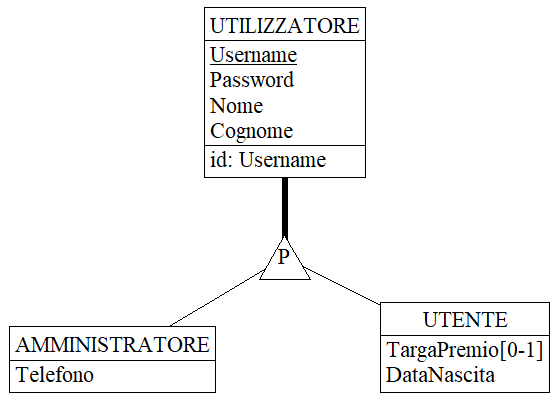
\includegraphics[width=300pt]{ER/utenza.png}
	\caption{Schema ER dell'utenza.}
\end{figure}
\subsection{Multimedia}
Qui viene descritto il concetto di \textbf{multimedia}(riferimento nella sezione \ref{ss:terminologia}), che si estende tramite generalizzazione alla rappresentazione di due sotto entità: \textbf{film} e \textbf{serie tv}. Un multimedia può essere associato a diversi \textbf{generi}, \textit{(quindi possono esistere, ad esempio, film/serie che sono sia horror che commedie)}, e l'inserimento dei generi è indipendente dall'esistenza dei multimedia, quindi si è optato per la cardinalità \textbf{0-N}. La principale differenza tra un film e una serie TV sta nel fatto che una serie può essere composta da più stagioni, ognuna con diversi episodi, mentre un film è un'unica narrazione senza interruzioni.
\begin{figure}[H]
	\centering
	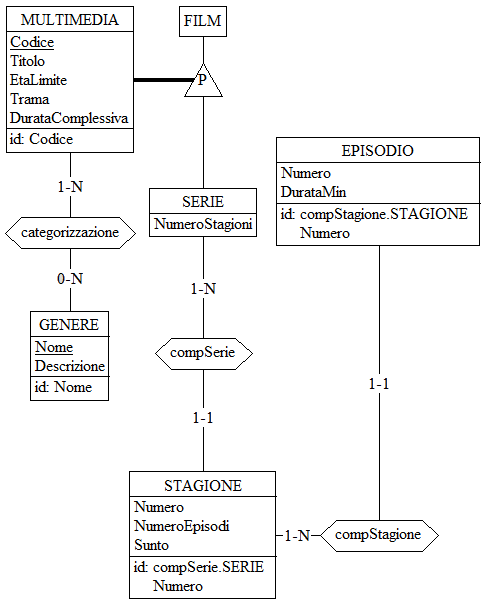
\includegraphics[width=300pt]{ER/multimedia.png}
	\caption{Schema ER dei multimedia.}
\end{figure}
\subsection{Cast}
I membri del cast da tracciare possono essere \textbf{registi} o \textbf{attori}; degli attori ci interessa in particolare un nome d'arte, mentre dei registi la data di debutto della carriera per effettuare delle statistiche. La generalizzazione in questo caso è \textit{totale} e \textit{sovrapposta}, questo significa che nel dominio del nostro problema non si vogliono tracciare altri membri oltre che a questi due, ed è sovrapposta perché possono esserci casi in cui un regista è anche un attore.
\begin{figure}[H]
	\centering
	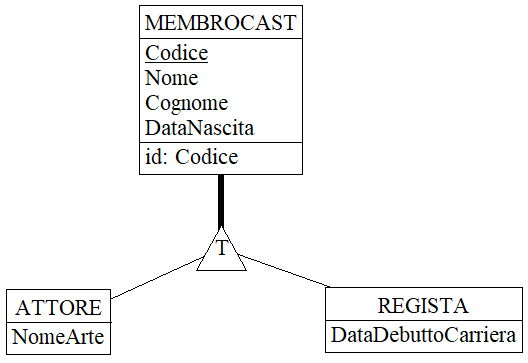
\includegraphics[width=300pt]{ER/cast.png}
	\caption{Schema ER dei membri del cast.}
\end{figure}
\subsection{Recensione}
Una recensione è suddivisa in più sezioni(ad esempio: trama, colonna sonora, etc\dots) e per ciascuna di esse viene assegnato un voto. Una sezione, invece, può esistere anche senza il concetto di recensione.
Il concetto di recensione si suddivide in due sottoconcetti, mediante una generalizzazione: recfilm (recensione di film) e recserie (recensione di serie TV). Entrambi sono identificati dall'utente che ha redatto la recensione, tuttavia recfilm è identificato anche dal film trattato, mentre recserie è identificata anche dalla serie televisiva.
\begin{figure}[H]
	\centering
	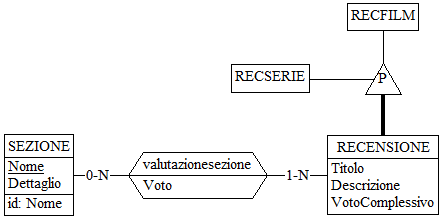
\includegraphics[width=300pt]{ER/recensione.png}
	\caption{Schema ER della recensione.}
\end{figure}
\subsection{Promo}
Una promozione è un'offerta limitata da una scadenza specifica, viene definita come un'istanza di un modello promozionale. Tale \textit{template} è caratterizzato da una percentuale di sconto, che gli utenti possono usufruire. La promo \textit{template} è suddivisa in due sotto entità in maniera totale ed esclusiva:
\begin{itemize}
	\item Singolo: valido per uno e un solo film.
	\item Multiplo: valido per uno o più generi di film.
\end{itemize}
\begin{figure}[H]
	\centering
	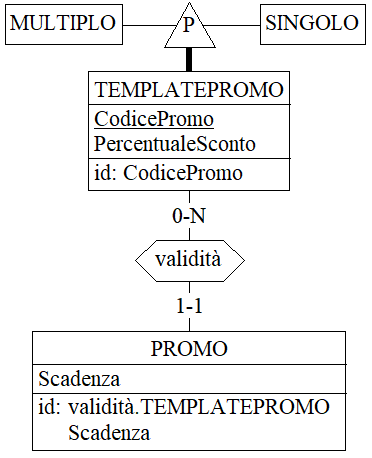
\includegraphics[width=270pt]{ER/promo.png}
	\caption{Schema ER della promo.}
\end{figure}
\subsection{Relazione tra utenza e recensioni}
Un utente può scrivere più di una recensione su vari film o serie tv, esplicitando il titolo, la descrizione della recensione e la sua valutazione. Quando viene scritta una recensione vengono scelti dei voti, ciascuno per ogni sezione selezionata dall'utente.
\begin{figure}[H]
	\centering
	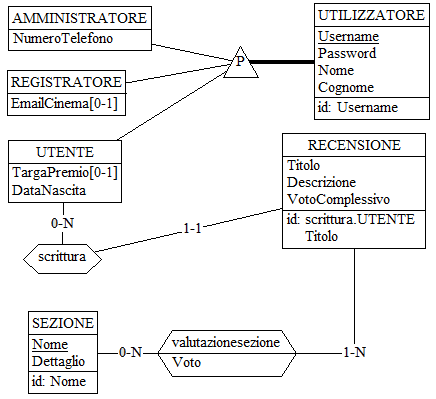
\includegraphics[width=300pt]{ER/utenzarecensione.png}
	\caption{Schema ER della relazione tra utenza e recensioni.}
\end{figure}
\subsection{Relazione tra utenza e cinema}
Un \textbf{cinema} afferisce a più registratori, mentre ciascuno di essi è a disposizione solo su di un cinema in particolare. Il \textbf{registratore} è considerato un \textbf{utilizzatore}, quindi è compreso nella generalizzazione.
\begin{figure}[H]
	\centering
	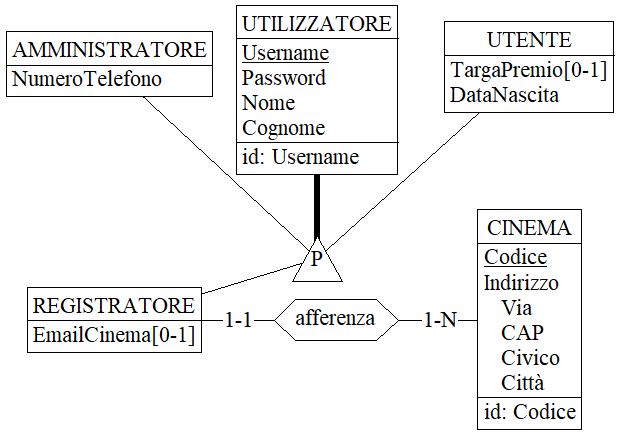
\includegraphics[width=300pt]{ER/utenzacinema.png}
	\caption{Schema ER della relazione tra utenza e cinema.}
\end{figure}
\subsection{Relazione tra utenza e tessera}
Gli utenti hanno la possibilità di iscriversi a una o più \textbf{tessere}. Una tessera è inserita da un \textbf{registratore}. Ciascuna tessera è caratterizzata da un numero univoco, che la identifica insieme all'utente tesserato, e da una data di rinnovo.
\begin{figure}[H]
	\centering
	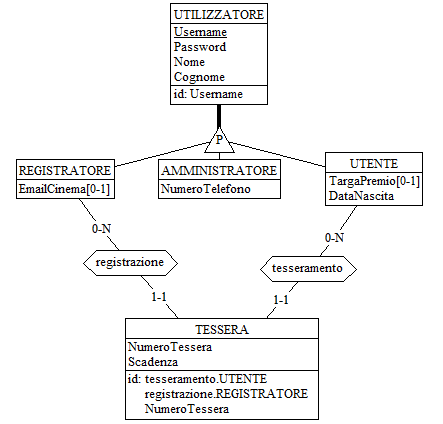
\includegraphics[width=300pt]{ER/utenzatessera.png}
	\caption{Schema ER della relazione tra utenza e tessera.}
\end{figure}
\subsection{Relazione tra multimedia e membri del cast}
Un \textbf{cast} può essere diretto da uno e un solo \textbf{regista} mentre possono prendere parte all'interno dello stesso uno o più \textbf{attori}. Queste due entità sono raggruppate tramite la generalizzazione "membro cast" che descrive un qualsiasi membro del cast cinematografico che ha presto parte nel film stesso.
Il cast è specifico per ogni singolo film, mentre può variare da stagione a stagione all'interno di una serie TV.
\begin{figure}[H]
	\centering
	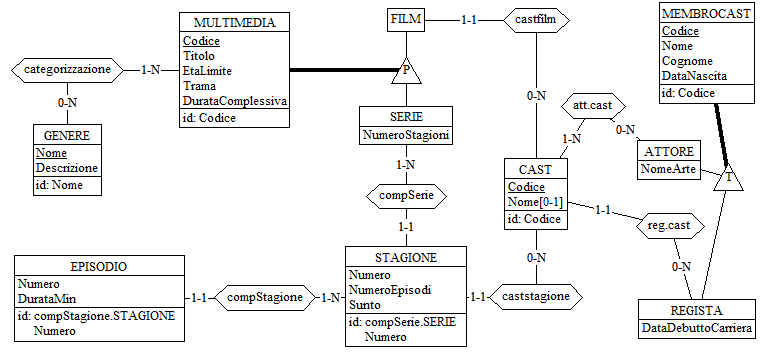
\includegraphics[width=350pt]{ER/multimediacast.png}
	\caption{Schema ER della relazione tra multimedia e membri del cast}
\end{figure}
\subsection{Relazione tra multimedia e promo}
Un multimedia può essere oggetto di offerte promozionali sia direttamente che tramite il suo genere. Il modello di promozione viene suddiviso in singolo e multiplo attraverso una generalizzazione, distinguendo il primo che è specifico del multimedia stesso, mentre il secondo si riferisce al genere.
\begin{figure}[H]
	\centering
	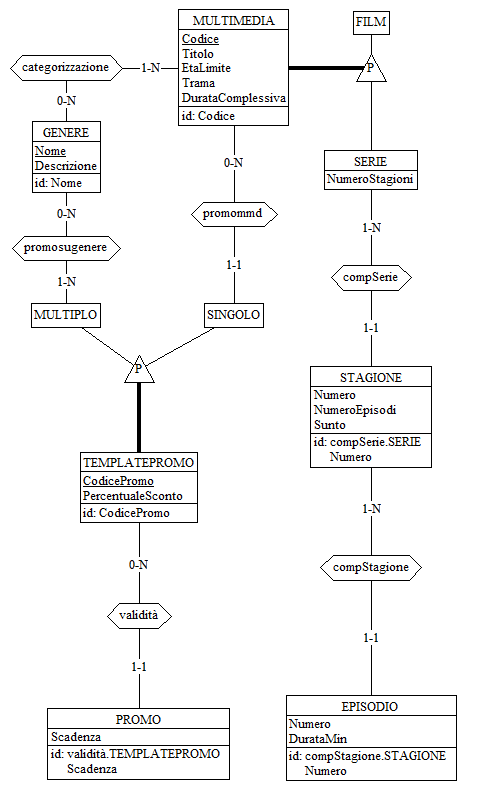
\includegraphics[width=300pt]{ER/multimediapromo.png}
	\caption{Schema ER della relazione tra multimedia e promo.}
\end{figure}
\subsection{Relazione tra multimedia, cast e promo}
Di un cast vengono memorizzati i membri che, mediante una generalizzazione, sono suddivisi in regista e attori. Il cast è associato a un film particolare o a una stagione di una serie TV. Queste due entità sono aggregate dal concetto di multimedia, il quale, come precedentemente descritto, è collegato al sistema di offerte promozionali.
\begin{figure}[H]
	\centering
	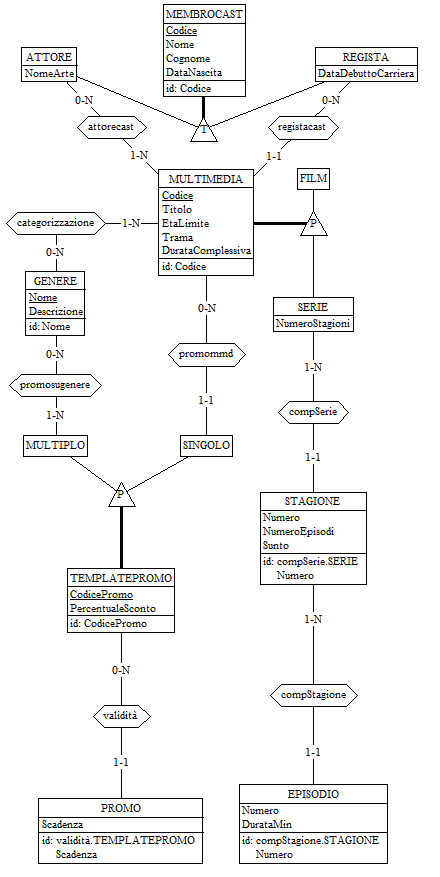
\includegraphics[width=300pt]{ER/multimediacastpromo.png}
	\caption{Schema ER della relazione tra multimedia, cast e promo.}
\end{figure}
\subsection{Relazione tra utenza, cinema, tessera e recensione}
Una tessera, inserita da un registratore per il cinema per cui lavora, può essere utilizzata da un utente che è stato premiato perché risultante particolarmente attivo sulla piattaforma. Questi utenti possono usufruire di vantaggi quali sconti e offerte per mezzo della tessera stessa. Nello specifico una tessera è valida solo per un cinema, quello di afferenza del registratore.
Inoltre includiamo il collegamento che vi è tra l'utenza e la recensione, che è stata precedentemente descritta.
\begin{figure}[H]
	\centering
	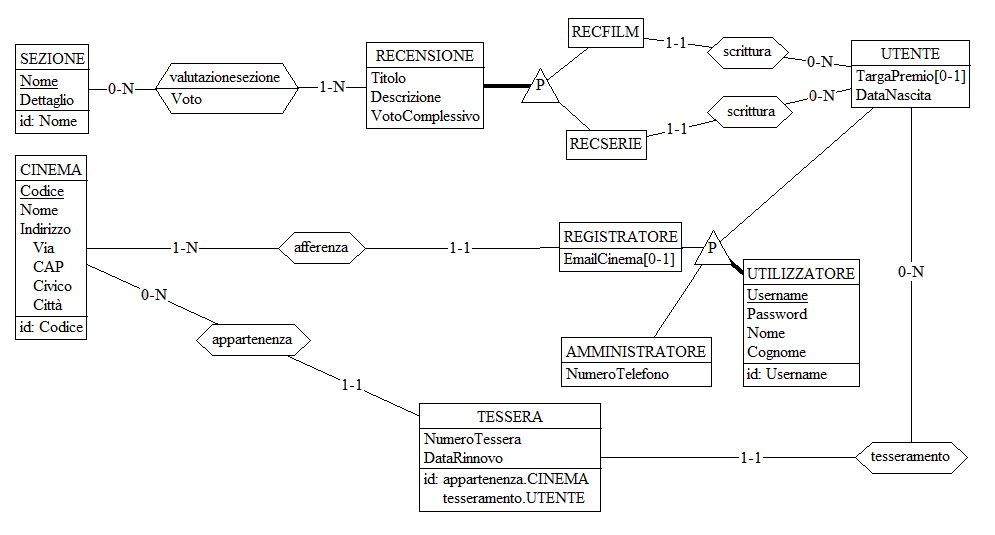
\includegraphics[width=450pt]{ER/utenzacinematesserarecensione.png}
	\caption{Schema ER della relazione tra utenza, cinema, tessera e recensione.}
\end{figure}
\subsection{Schema completo}
Quello che segue rappresenta lo schema derivato dalla composizione di tutte le sotto-componenti descritte precedentemente.
\begin{figure}[H]
	\centering
	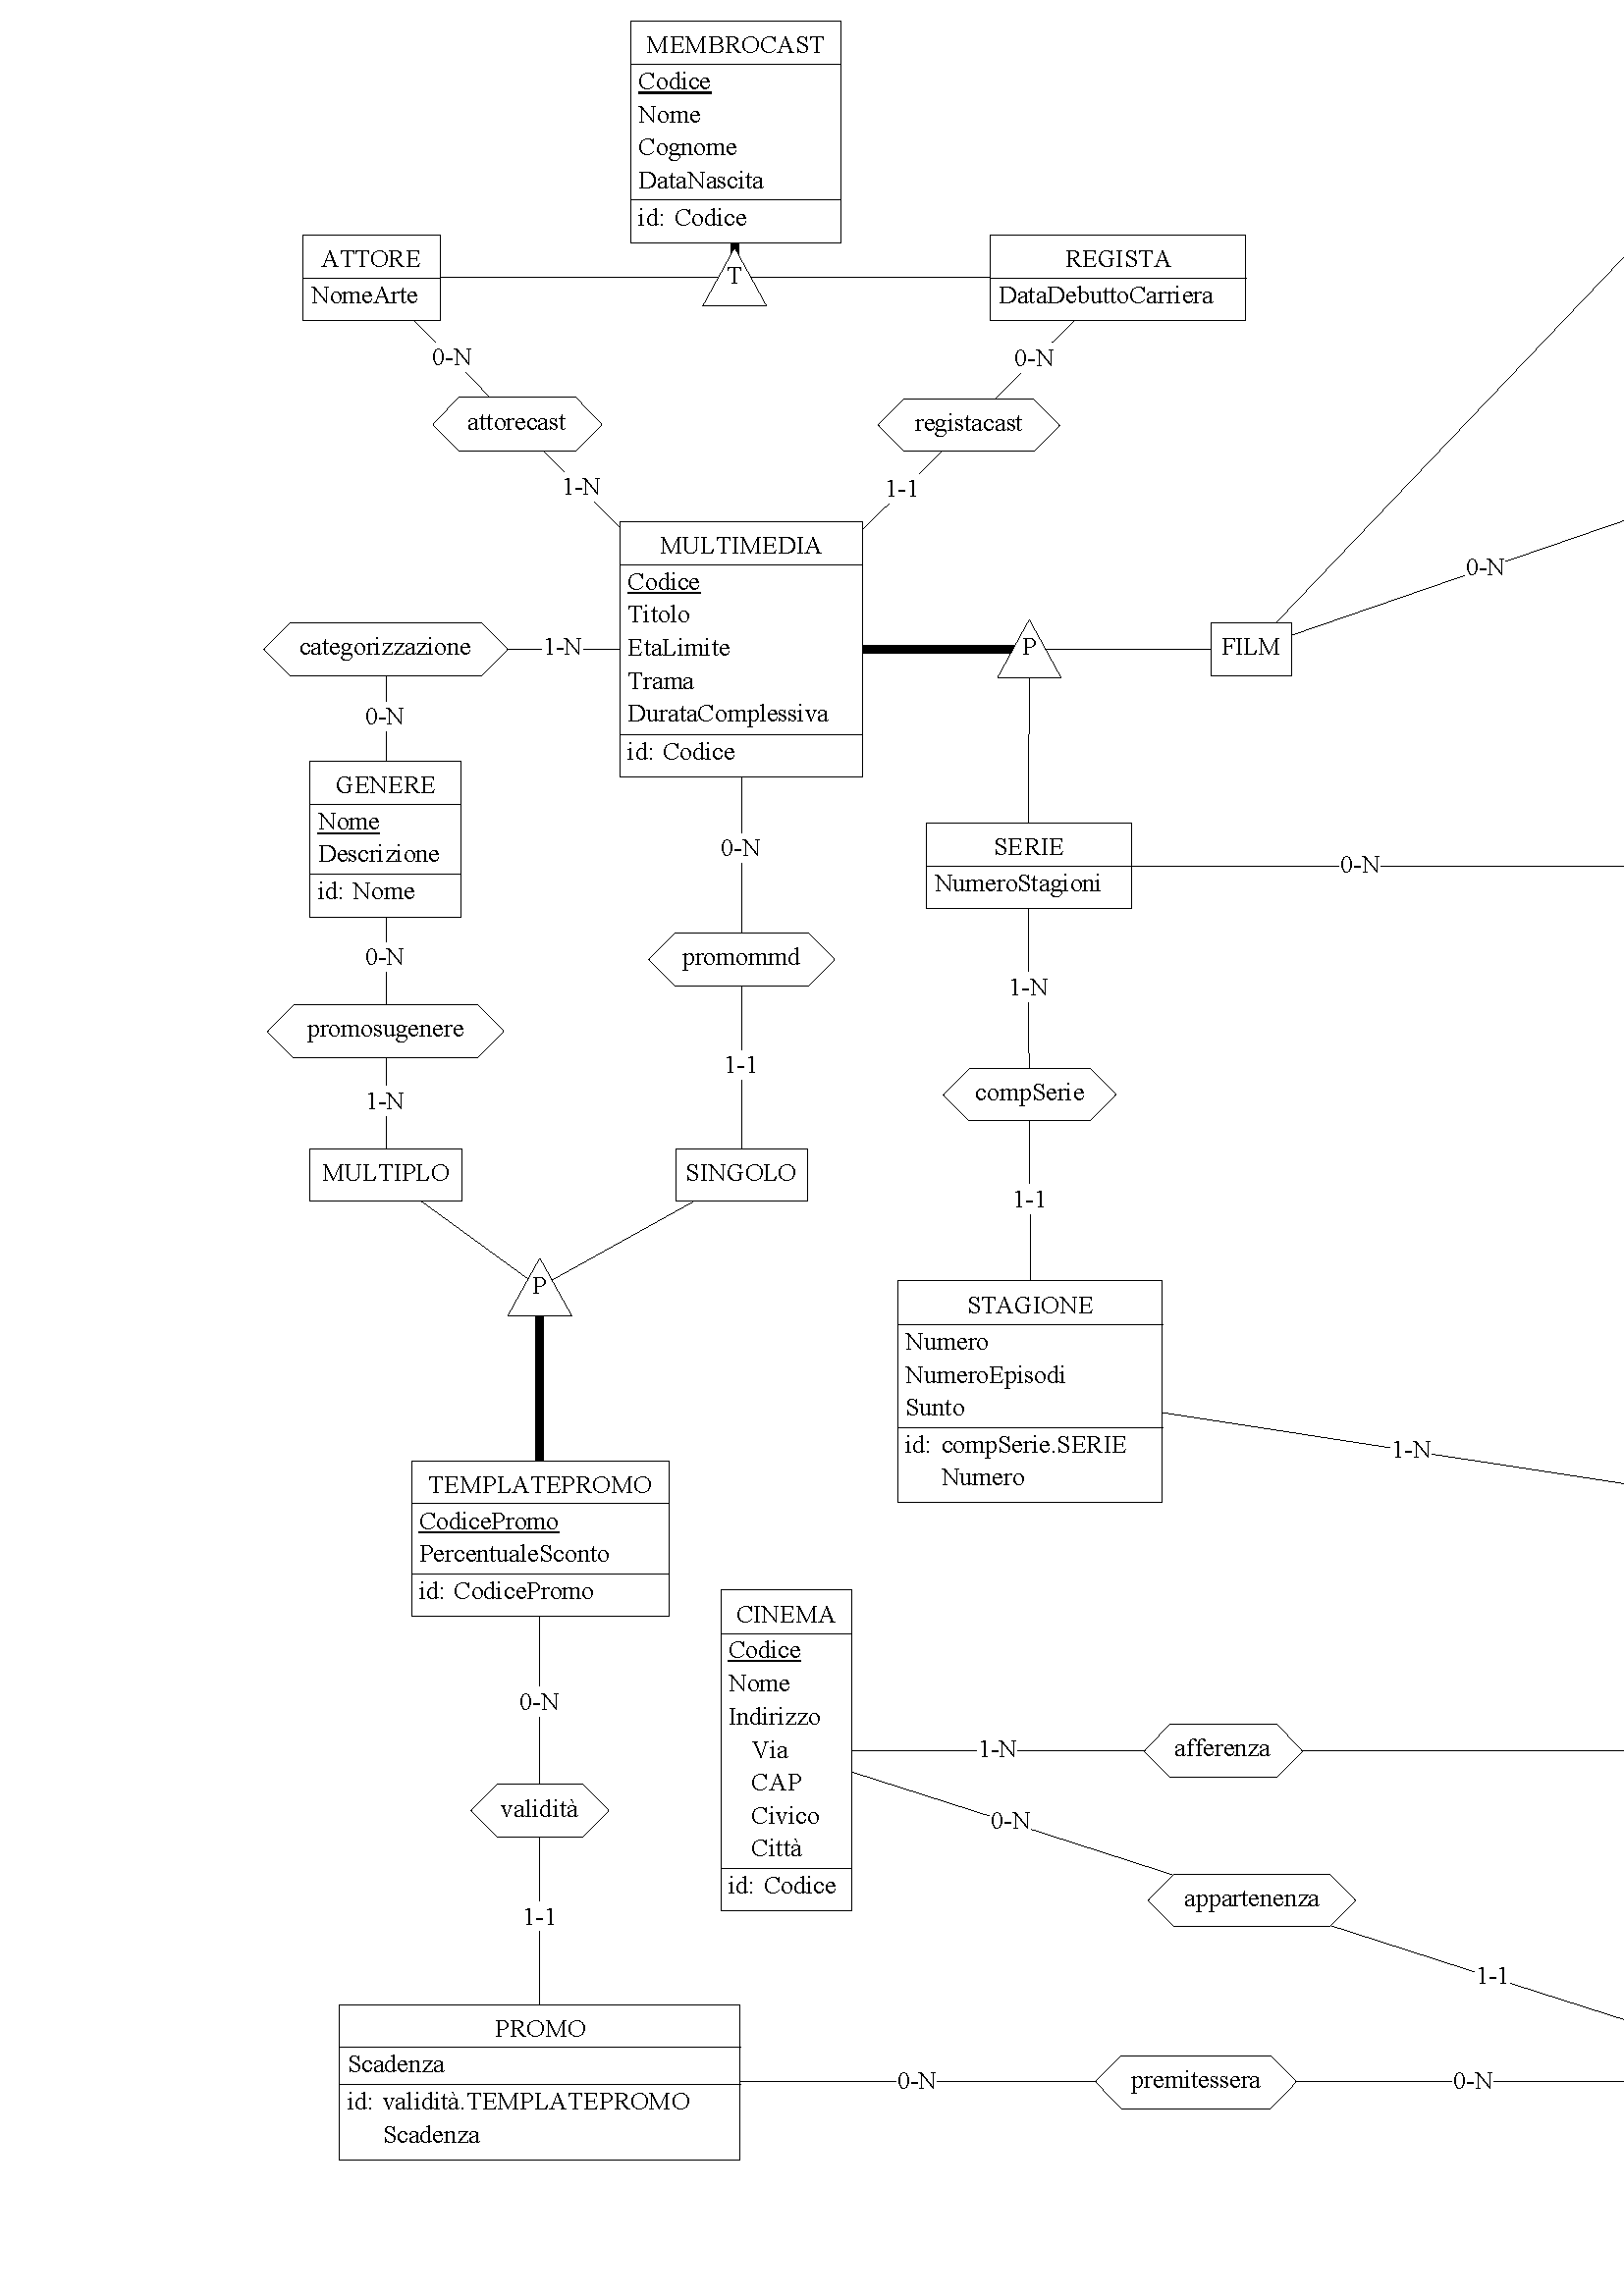
\includegraphics[width=450pt]{ER/ercompletosx.png}
	\caption{Schema ER completo \textbf{1/2}.}
\end{figure}
\begin{figure}[H]
	\centering
	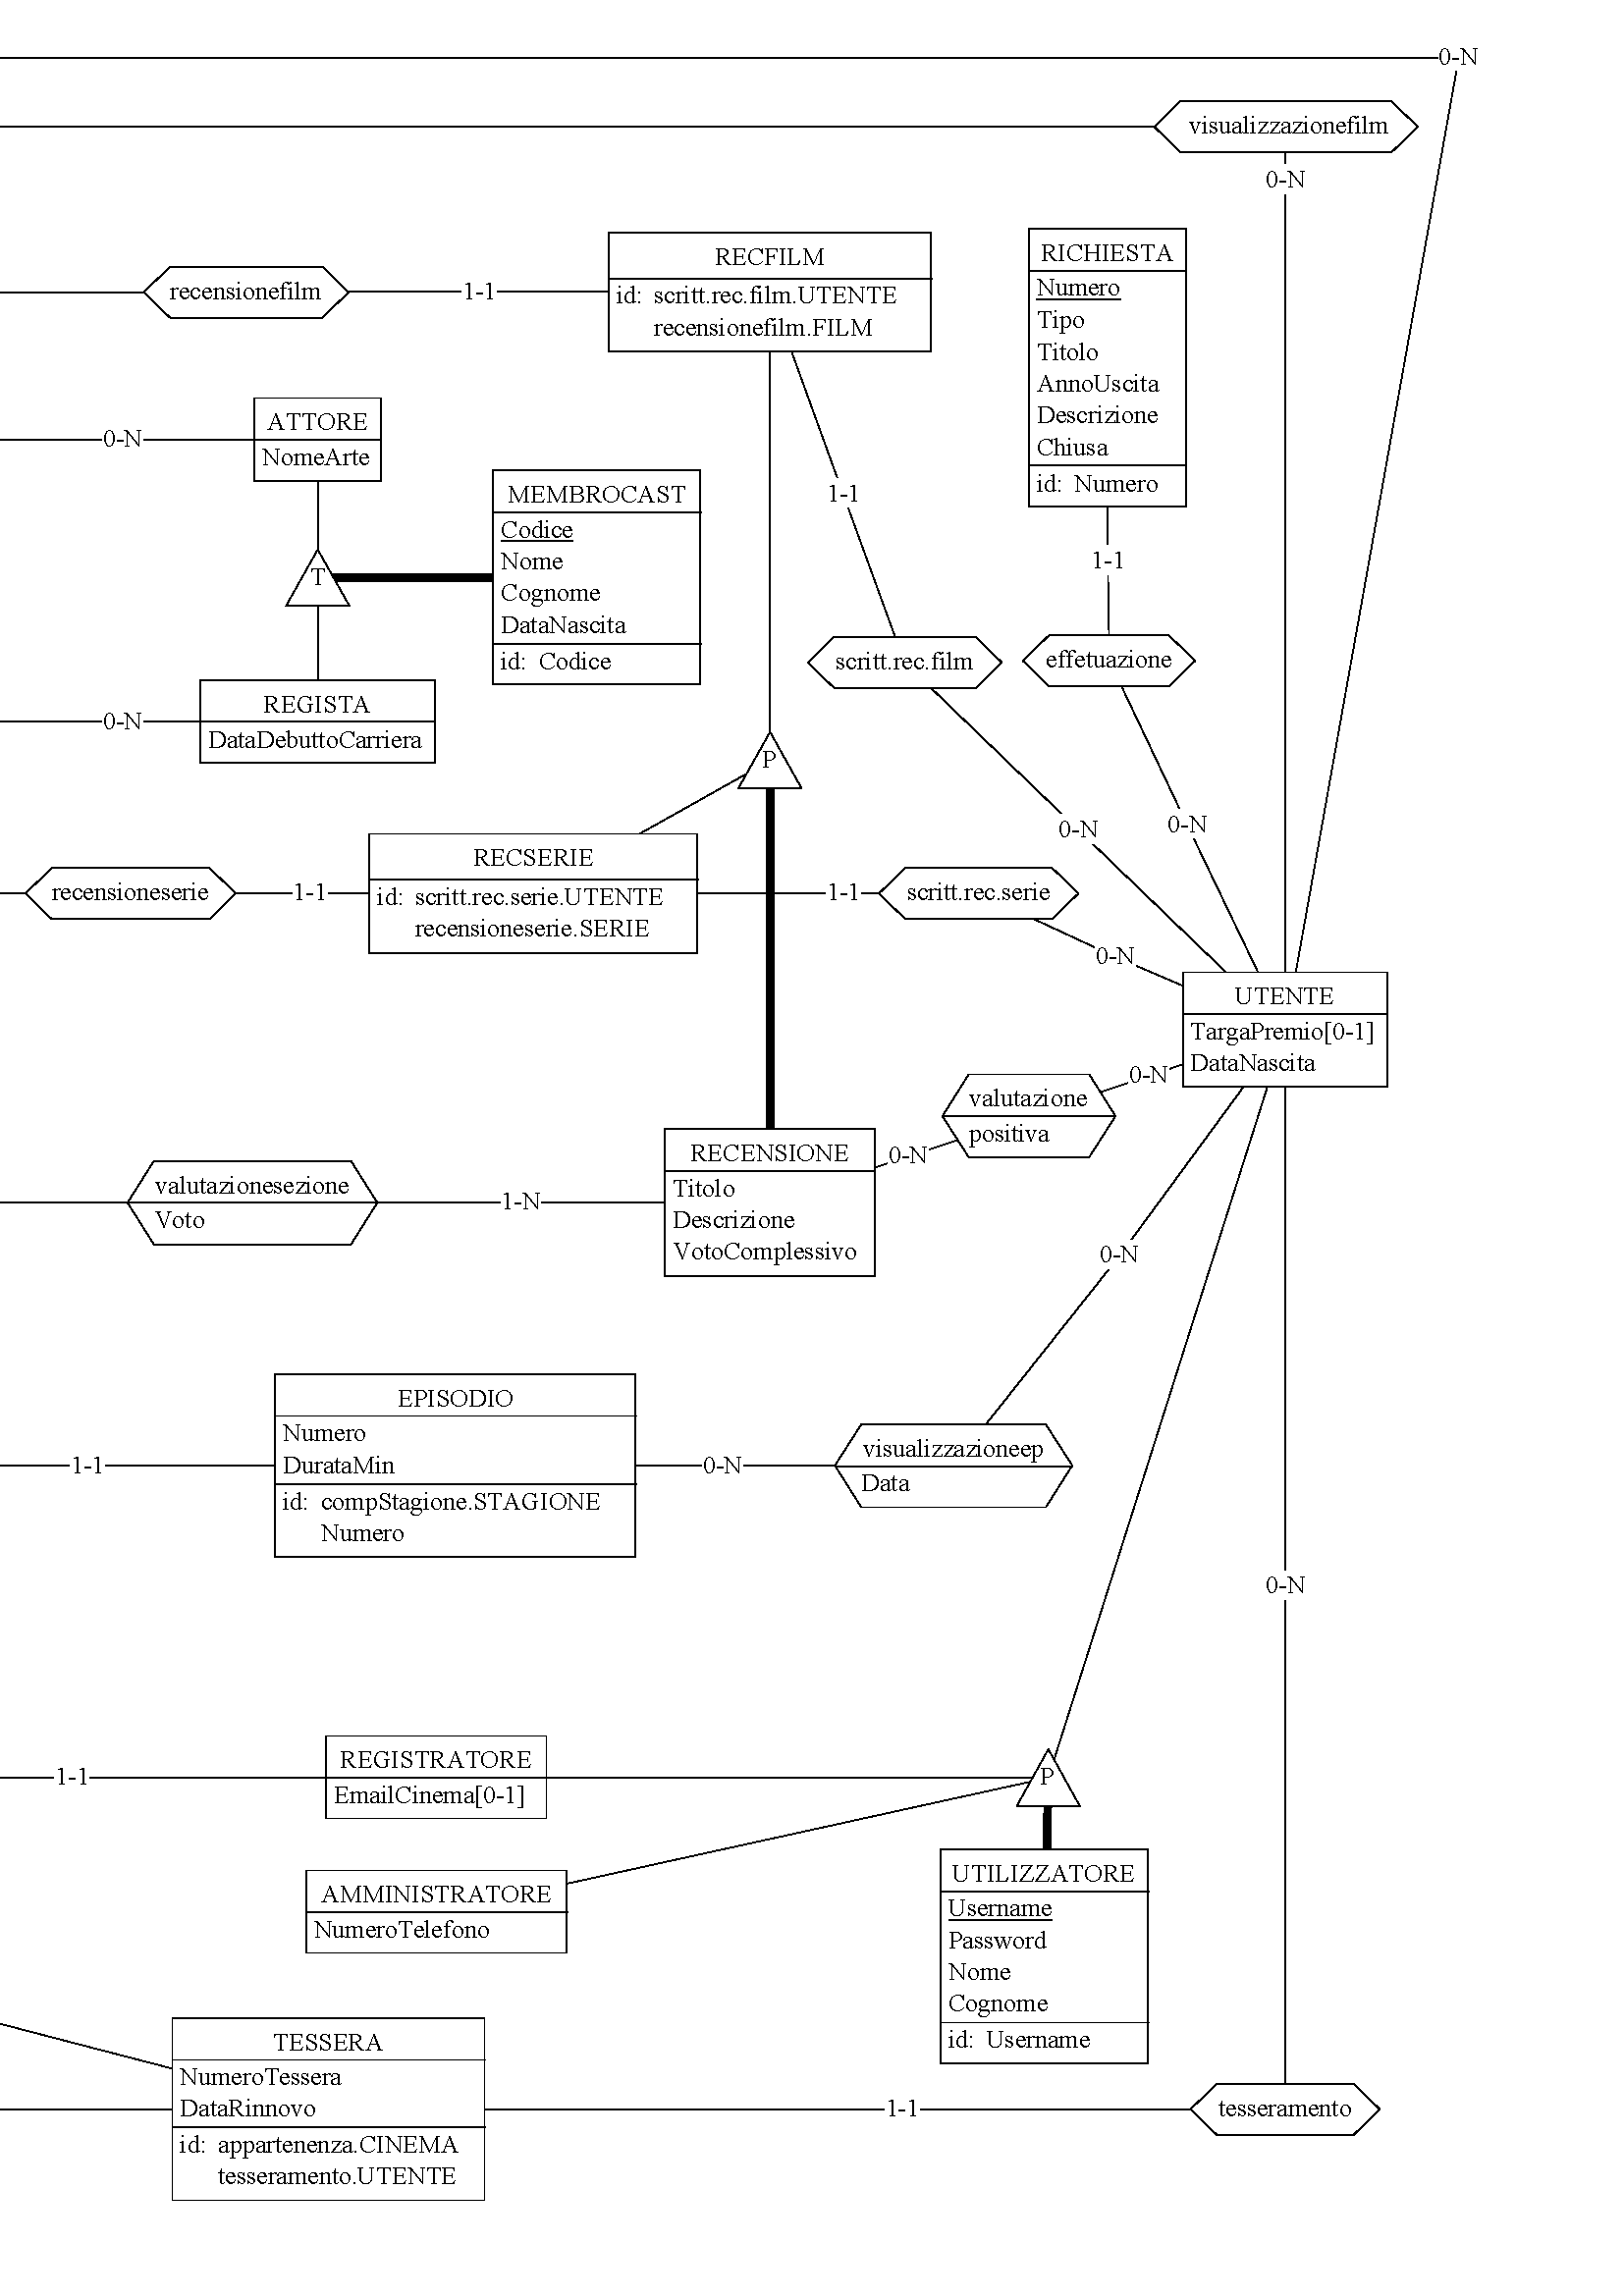
\includegraphics[width=450pt]{ER/ercompletodx.png}
	\caption{Schema ER completo \textbf{2/2}.}
\end{figure}
\chapter{Progettazione Logica}
\section{Stima del volume dei dati} \label{s:volumes}
\begin{table}[H]
	\centering
	\begin{tabular}{|lll|}
		\hline
		\rowcolor[HTML]{FFCE93}
		\multicolumn{3}{|l|}{\cellcolor[HTML]{FFCE93}Film} \\ \hline
		\rowcolor[HTML]{CBCEFB}
		Concetto            & Costrutto & Volume           \\ \hline
		MULTIMEDIA          & E         & 12000            \\ \hline
		FILM                & E         & 9500             \\ \hline
		SERIE               & E         & 2500             \\ \hline
		GENERE              & E         & 13               \\ \hline
		categorizzazione    & R         & 50000            \\ \hline
		visualizzazionefilm & R         & 350000           \\ \hline
		preferenza          & R         & 29880            \\ \hline
	\end{tabular}
\end{table}
\begin{table}[H]
	\centering
	\begin{tabular}{|lll|}
		\hline
		\rowcolor[HTML]{FFCE93}
		\multicolumn{3}{|l|}{\cellcolor[HTML]{FFCE93}Cast} \\ \hline
		\rowcolor[HTML]{CBCEFB}
		Concetto    & Costrutto & Volume                   \\ \hline
		ATTORE      & E         & 5200                     \\ \hline
		REGISTA     & E         & 600                      \\ \hline
		CAST        & E         & 12000                    \\ \hline
		attorecast  & R         & 12000                    \\ \hline
		registacast & R         & 12000                    \\ \hline
	\end{tabular}
\end{table}
\begin{table}[H]
	\centering
	\begin{tabular}{|lll|}
		\hline
		\rowcolor[HTML]{FFCE93}
		\multicolumn{3}{|l|}{\cellcolor[HTML]{FFCE93}Serie TV} \\ \hline
		\rowcolor[HTML]{CBCEFB}
		Concetto          & Costrutto & Volume                 \\ \hline
		STAGIONE          & E         & 10000                  \\ \hline
		EPISODIO          & E         & 400000                 \\ \hline
		compstagione      & R         & 400000                 \\ \hline
		compserie         & R         & 10000                  \\ \hline
		visualizzazioneep & R         & 1400000                \\ \hline
	\end{tabular}
\end{table}
\begin{table}[H]
	\centering
	\begin{tabular}{|lll|}
		\hline
		\rowcolor[HTML]{FFCE93}
		\multicolumn{3}{|l|}{\cellcolor[HTML]{FFCE93}Utilizzatori} \\ \hline
		\rowcolor[HTML]{CBCEFB}
		Concetto       & Costrutto & Volume                        \\ \hline
		UTILIZZATORE   & E         & 10000                         \\ \hline
		AMMINISTRATORE & E         & 10                            \\ \hline
		REGISTRATORE   & E         & 30                            \\ \hline
		UTENTE         & E         & 9960                          \\ \hline
	\end{tabular}
\end{table}
\begin{table}[H]
	\centering
	\begin{tabular}{|lll|}
		\hline
		\rowcolor[HTML]{FFCE93}
		\multicolumn{3}{|l|}{\cellcolor[HTML]{FFCE93}Cinema e registratori di tessere} \\ \hline
		\rowcolor[HTML]{CBCEFB}
		Concetto     & Costrutto & Volume                                              \\ \hline
		CINEMA       & E         & 25                                                  \\ \hline
		TESSERA      & E         & 3500                                                \\ \hline
		appartenenza & R         & 3500                                                \\ \hline
		tesseramento & R         & 3500                                                \\ \hline
		afferenza    & R         & 30                                                  \\ \hline
	\end{tabular}
\end{table}
\begin{table}[H]
	\centering
	\begin{tabular}{|lll|}
		\hline
		\rowcolor[HTML]{FFCE93}
		\multicolumn{3}{|l|}{\cellcolor[HTML]{FFCE93}Coupon e premi su tessera} \\ \hline
		\rowcolor[HTML]{CBCEFB}
		Concetto       & Costrutto & Volume                                     \\ \hline
		PROMO          & E         & 200                                        \\ \hline
		TEMPLATEPROMO  & E         & 500                                        \\ \hline
		MULTIPLO       & E         & 25                                         \\ \hline
		SINGOLO        & E         & 475                                        \\ \hline
		premitessera   & R         & 1500                                       \\ \hline
		validità       & R         & 200                                        \\ \hline
		couponsugenere & R         & 50                                         \\ \hline
		couponsufilm   & R         & 475                                        \\ \hline
	\end{tabular}
\end{table}
\begin{table}[H]
	\centering
	\begin{tabular}{|lll|}
		\hline
		\rowcolor[HTML]{FFCE93}
		\multicolumn{3}{|l|}{\cellcolor[HTML]{FFCE93}Recensioni} \\ \hline
		\rowcolor[HTML]{CBCEFB}
		Concetto                 & Costrutto & Volume            \\ \hline
		RECENSIONE               & E         & 1200000           \\ \hline
		SEZIONE                  & E         & 5                 \\ \hline
		recensionefilm           & R         & 950000            \\ \hline
		recensioneserie          & R         & 250000            \\ \hline
		valutazione              & R         & 115000            \\ \hline
		valutazionesezione       & R         & 1400000           \\ \hline
		scritturarecensionefilm  & R         & 950000            \\ \hline
		scritturarecensioneserie & R         & 250000            \\ \hline
	\end{tabular}
\end{table}
\section{Operazioni e loro frequenza}
\subsection{Operazioni dell'utenza}
\begin{longtable}[H]{|c|c|>{\columncolor[HTML]{FFFFC7}}c |c|}
	\hline
	\cellcolor[HTML]{ECF4FF}Numero                                                                                                                                                                               &
	\cellcolor[HTML]{ECF4FF}Operazione                                                                                                                                                                           &
	\cellcolor[HTML]{ECF4FF}Frequenza / gg                                                                                                                                                                       &
	\cellcolor[HTML]{ECF4FF}Dettagli                                                                                                                                                                                                                                                                         \\ \hline
	\endfirsthead
	%
	\endhead
	%
	1                                                                                                                                                                                                            &
	\begin{tabular}[c]{@{}c@{}}Registrazione di \\ un nuovo utente.\end{tabular}                                                                                                                                 &
	2                                                                                                                                                                                                            &
	\\ \hline
	2.1                                                                                                                                                                                                          &
	\begin{tabular}[c]{@{}c@{}}Accesso di un \\ utente.\end{tabular}                                                                                                                                             &
	100                                                                                                                                                                                                          &
	\\ \hline
	2.2                                                                                                                                                                                                          &
	\begin{tabular}[c]{@{}c@{}}Accesso di un \\ amministratore.\end{tabular}                                                                                                                                     &
	2                                                                                                                                                                                                            &
	\\ \hline
	2.3                                                                                                                                                                                                          &
	\begin{tabular}[c]{@{}c@{}}Accesso di un \\ registratore.\end{tabular}                                                                                                                                       &
	5                                                                                                                                                                                                            &
	\\ \hline
	3.1                                                                                                                                                                                                          &
	Scelta delle preferenze.                                                                                                                                                                                     &
	2                                                                                                                                                                                                            &
	Solo in fase di registrazione                                                                                                                                                                                                                                                                            \\ \hline
	3.2                                                                                                                                                                                                          &
	\begin{tabular}[c]{@{}c@{}}Aggiornamento \\ delle preferenze.\end{tabular}                                                                                                                                   &
	15                                                                                                                                                                                                           &
	\begin{tabular}[c]{@{}c@{}}Tra tutti gli utenti \\ che accedano in un \\ giorno, è plausibile \\ che pochi aggiornino \\ le proprie preferenze.\end{tabular}                                                                                                                                             \\ \hline
	4.1                                                                                                                                                                                                          &
	\begin{tabular}[c]{@{}c@{}}Visualizzare tutto \\ l'elenco dei film \\ in base all'età \\ di chi lo richiede.\end{tabular}                                                                                    &
	100                                                                                                                                                                                                          &
	\begin{tabular}[c]{@{}c@{}}Viene effettuato all'accesso.\end{tabular}                                                                                                                                                                                                                                    \\ \hline
	4.2                                                                                                                                                                                                          &
	\begin{tabular}[c]{@{}c@{}}Visualizzare l'elenco \\ dei film in base\\ ad un'età scelta.\end{tabular}                                                                                                        &
	17                                                                                                                                                                                                           &
	\begin{tabular}[c]{@{}c@{}}Meno frequenza \\ rispetto all'operazione\\ precedente, \\ i genitori registrati che\\ accedono ed usano \\ questa funzione sono\\ meno.\end{tabular}                                                                                                                         \\ \hline
	4.3                                                                                                                                                                                                          &
	\begin{tabular}[c]{@{}c@{}}Visualizzare l'elenco \\ delle serie TV \\ con la relativa \\ durata complessiva \\ e il numero  di stagioni \\ ed episodi complessivo, \\ in base all'età \\ di chi lo richiede.\end{tabular} &
	100                                                                                                                                                                                                          &
	\begin{tabular}[c]{@{}c@{}}Viene effettuato all'accesso.\end{tabular}                                                                                                                                                                                                                                    \\ \hline
	4.4                                                                                                                                                                                                          &
	\begin{tabular}[c]{@{}c@{}}Visualizzare le \\ informazioni riguardanti \\ una serie TV, comprese \\ tutte le stagioni \\ e tutti gli episodi.\end{tabular}                                                   &
	50                                                                                                                                                                                                           &
	\\ \hline
	4.5                                                                                                                                                                                                          &
	\begin{tabular}[c]{@{}c@{}}Aggiunta di una \\ nuova stagione per una \\ specifica serie TV.\end{tabular}                                                 &
	5																						&
	
	\\ \hline
	4.6                                                                                                                                                                                                          &
	\begin{tabular}[c]{@{}c@{}}Aggiunta di un \\ nuovo episodio per una \\ specifica stagione di una serie TV.\end{tabular}                                                   &
	10																						&
	
	\\ \hline
	5.1                                                                                                                                                                                                          &
	\begin{tabular}[c]{@{}c@{}}Contrassegnare \\ come "visualizzato" \\ un film.\end{tabular}                                                                                                                    &
	350                                                                                                                                                                                                          &
	\begin{tabular}[c]{@{}c@{}}Considerando che in \\ genere chi accede\\ all'applicativo e vede \\ la lista dei film,\\ scrive una recensione \\ su almeno un film,\\ implica che l'abbia \\ precedentemente\\ visualizzato. \\ Potrebbe essere \\ che venga contrassegnato \\ più di un film.\end{tabular} \\ \hline
	5.2                                                                                                                                                                                                          &
	\begin{tabular}[c]{@{}c@{}}Contrassegnare \\ come "visualizzato" \\ un episodio \\ di una serie.\end{tabular}                                                                                                &
	500                                                                                                                                                                                                          &                                                                                           \\ \hline
	6                                                                                                                                                                                                            &
	Recensire un film.                                                                                                                                                                                           &
	20                                                                                                                                                                                                           &
	\begin{tabular}[c]{@{}c@{}}Dei film contrassegnati \\ in un giorno solo\\ alcuni verranno recensiti.\end{tabular}                                                                                                                                                                                        \\ \hline
	7.1                                                                                                                                                                                                          &
	\begin{tabular}[c]{@{}c@{}}Visualizzare le \\ recensioni di un film.\end{tabular}                                                                                                                            &
	250                                                                                                                                                                                                           &
	\\ \hline
	7.2                                                                                                                                                                                                          &
	\begin{tabular}[c]{@{}c@{}}Dare una valutazione \\ di utilità ad una\\ recensione di un altro \\ utente su un film.\end{tabular}                                                                             &
	40                                                                                                                                                                                                           &
	\\ \hline
	7.3                                                                                                                                                                                                          &
	\begin{tabular}[c]{@{}c@{}}Dare una valutazione \\ di utilità ad una\\ recensione di un altro \\ utente su una serie.\end{tabular}                                                                           &
	30                                                                                                                                                                                                           &
	\\ \hline
	7.4                                                                                                                                                                                                          &
	\begin{tabular}[c]{@{}c@{}}Visualizzare le \\ recensioni di una \\ singola serie.\end{tabular}                                                                                                               &
	150                                                                                                                                                                                                           &
	\\ \hline
	7.5                                                                                                                                                                                                          &
	\begin{tabular}[c]{@{}c@{}}Aggiornare il voto \\ di una sezione \\ di una recensione.\end{tabular}                                                                                                               &
	50                                                                                                                                                                                                           &
	\\ \hline
	8.1                                                                                                                                                                                                          &
	\begin{tabular}[c]{@{}c@{}}Ottenere una \\ classifica dei generi\\ più visualizzati.\end{tabular}                                                                                                            &
	5                                                                                                                                                                                                            &
	\begin{tabular}[c]{@{}c@{}}Si considera nella \\ classifica solo la serie \\ completa come visualizzata, \\ se si visualizza \\ un singolo episodio \\ senza completare la \\ serie di appartenenza,\\ questo non verrà\\ considerato nel conteggio\\ per le visualizzazioni\\ dei generi.\end{tabular}
	\\ \hline
	8.2                                                                                                                                                                                                          &
	\begin{tabular}[c]{@{}c@{}}Visualizzare una \\ classifica dei registi in\\ base alla media \\ delle recensioni.\end{tabular}                                                                                 &
	6                                                                                                                                                                                                            &
	\\ \hline
\end{longtable}
\subsection{Operazioni di amministrazione}
\begin{longtable}[H]{|c|c|>{\columncolor[HTML]{FFFFC7}}c |c|}
	\hline
	\cellcolor[HTML]{ECF4FF}Numero                                                                                                                                                   &
	\cellcolor[HTML]{ECF4FF}Operazione                                                                                                                                               &
	\cellcolor[HTML]{ECF4FF}Frequenza                                                                                                                                                &
	\cellcolor[HTML]{ECF4FF}Dettagli                                                                                                                                                                 \\ \hline
	\endfirsthead
	%
	\endhead
	%
	9.1                                                                                                                                                                              &
	\begin{tabular}[c]{@{}c@{}}Reperimento della\\ classifica degli \\ utenti con la media\\ delle valutazioni di\\ utilità sulle proprie\\ recensioni peggiore.\end{tabular}        &
	1 / mese                                                                                                                                                                         &
	\\ \hline
	9.2                                                                                                                                                                              &
	\begin{tabular}[c]{@{}c@{}}Come 9.1 ma è la\\ media delle recensioni\\ migliori.\end{tabular}                                                                                    &
	1 / settimana                                                                                                                                                                    &
	\begin{tabular}[c]{@{}c@{}}La premiazione degli\\ utenti con dei coupon\\ è settimanale.\end{tabular}                                                                                            \\ \hline
	10                                                                                                                                                                               &
	\begin{tabular}[c]{@{}c@{}}Assegnamento in blocco \\ di una promozione\\ ai primi 5 utenti tesserati \\ che si trovano in cima alla\\ classifica stilata (vedi 9.2)\end{tabular} &
	5 / settimana                                                                                                                                                                    &
	\\ \hline
	11.1                                                                                                                                                                             &
	\begin{tabular}[c]{@{}c@{}}Aggiunta di un nuovo \\ film alla piattaforma.\end{tabular}                                                                                           &
	4 / giorno                                                                                                                                                                       &
	\begin{tabular}[c]{@{}c@{}}Escono circa 2000 film \\ all'anno in tutto il mondo, \\ supponendo che si \\ aggiungano tutti i film\\ appena escono, vengono\\ circa 4 film al giorno.\end{tabular} \\ \hline
	11.2                                                                                                                                                                             &
	\begin{tabular}[c]{@{}c@{}}Aggiunta di persone che\\ hanno realizzato un film\\ alla piattaforma\end{tabular}                                                                    &
	664 / mese                                                                                                                                                                       &
	\begin{tabular}[c]{@{}c@{}}Considerando una stima\\ di 4 membri rilevanti del\\ cast di un film che si\\ vogliono tracciare, regista\\ compreso.\end{tabular}                                    \\ \hline
\end{longtable}
\subsection{Operazioni del registratore}
\begin{longtable}[H]{|c|c|>{\columncolor[HTML]{FFFFC7}}c |c|}
	\hline
	\cellcolor[HTML]{ECF4FF}Numero                                                   &
	\cellcolor[HTML]{ECF4FF}Operazione                                               &
	\cellcolor[HTML]{ECF4FF}Frequenza                                                &
	\cellcolor[HTML]{ECF4FF}Dettagli                                                   \\ \hline
	\endfirsthead
	%
	\endhead
	%
	12                                                                               &
	\begin{tabular}[c]{@{}c@{}}Registrazione di \\ una nuova \\ tessera\end{tabular} &
	20 / giorno                                                                      &
	\\ \hline
\end{longtable}
\section{Raffinamento dello schema}
\subsection{Eliminazione delle gerarchie}
\subsubsection{	Gerarchia "Multimedia"}
Questa gerarchia è stata risolta adottando il metodo del collasso verso il basso, questo perché l'accesso alle entità avviene separatamente (i film vengono reperiti in maniera separata dalle serie e viceversa). Questo metodo è inoltre applicabile perché la copertura della gerarchia è totale ed esclusiva.
\begin{figure}[H]
	\centering
	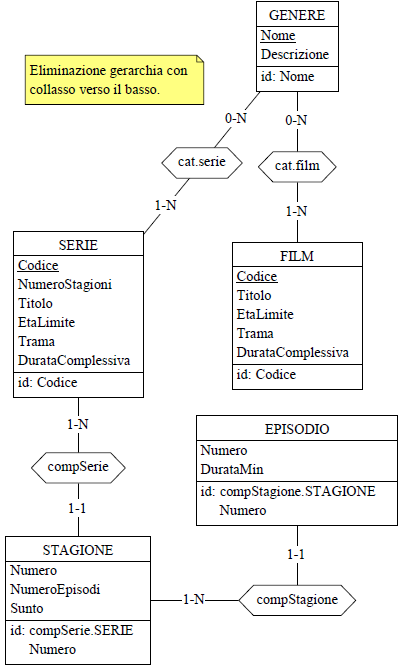
\includegraphics{ER/ristrutturazione/ristmultimedia.png}
	\caption{Ristrutturazione della gerarchia "Multimedia"}
\end{figure}
\subsubsection{Gerarchia "Recensione"}
Analogamente alla precedente, è stato usato il collasso verso il basso.
\begin{figure}[H]
	\centering
	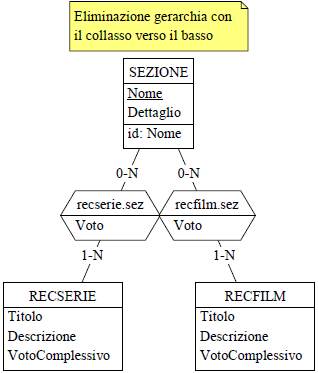
\includegraphics{ER/ristrutturazione/ristrecensione.png}
	\caption{Ristrutturazione della gerarchia "Recensione"}
\end{figure}
\subsubsection{Gerarchia "Membro Cast"}
In questo caso abbiamo una copertura totale ma sovrapposta, e dato che in genere quando si consulta il cast di un film, che è una consultazione più frequente rispetto al reperimento di un singolo attore o regista, si accedono entrambi i tipi di membri del cast contemporaneamente, per questo si è optato per il collasso verso l'alto con selettori di tipo (copertura sovrapposta).
\begin{figure}[H]
	\centering
	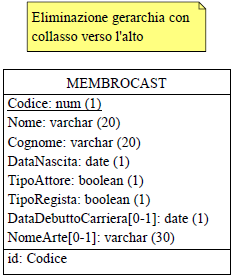
\includegraphics{ER/ristrutturazione/ristmembrocast.png}
	\caption{Ristrutturazione della gerarchia "Membro cast"}
\end{figure}
\subsubsection{Gerarchia "Template Promo"}
Questa gerarchia è stata rielaborata mantenendo le entità e introducendo delle relazione al posto della gerarchia, questo perché vi è copertura totale ed esclusiva e ci sono relazioni distinte sia con il padre che con le entità figlie.
\begin{figure}[H]
	\centering
	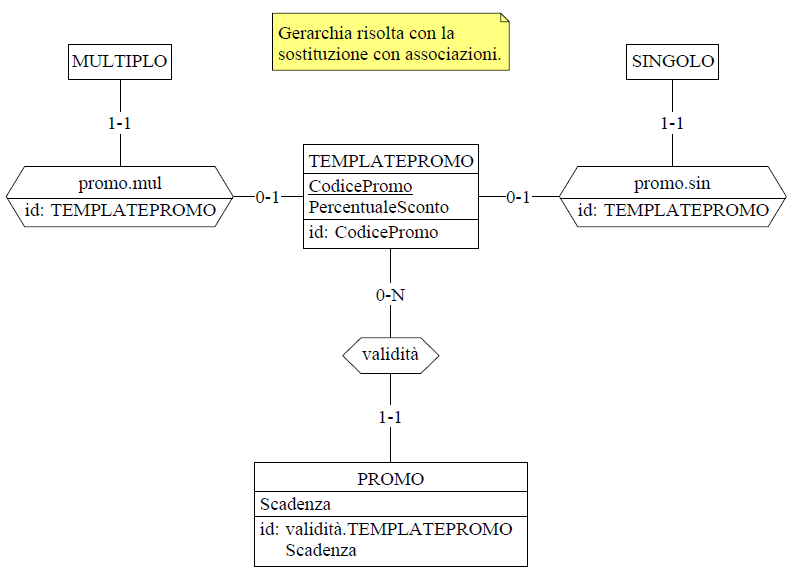
\includegraphics[width=400pt]{ER/ristrutturazione/ristpromo.png}
	\caption{Ristrutturazione della gerarchia "Template Promo"}
\end{figure}
\subsubsection{Gerarchia "Utilizzatore"}
Analogamente alla precedente, è stato usato il mantenimento delle gerarchie (Se si fosse utilizzato il collasso verso il basso i nomi utente non sarebbero stati univoci tra i diversi tipi di utente).
\begin{figure}[H]
	\centering
	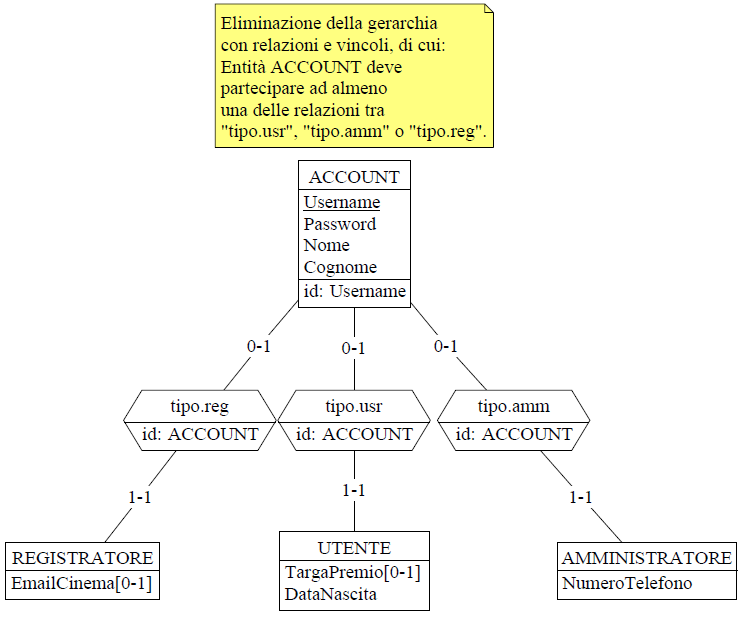
\includegraphics{ER/ristrutturazione/ristutenza.png}
	\caption{Ristrutturazione della gerarchia "Utilizzatore"}
\end{figure}
\subsubsection{Schema completo dopo l'eliminazione delle gerarchie}
\begin{figure}[H]
	\centering
	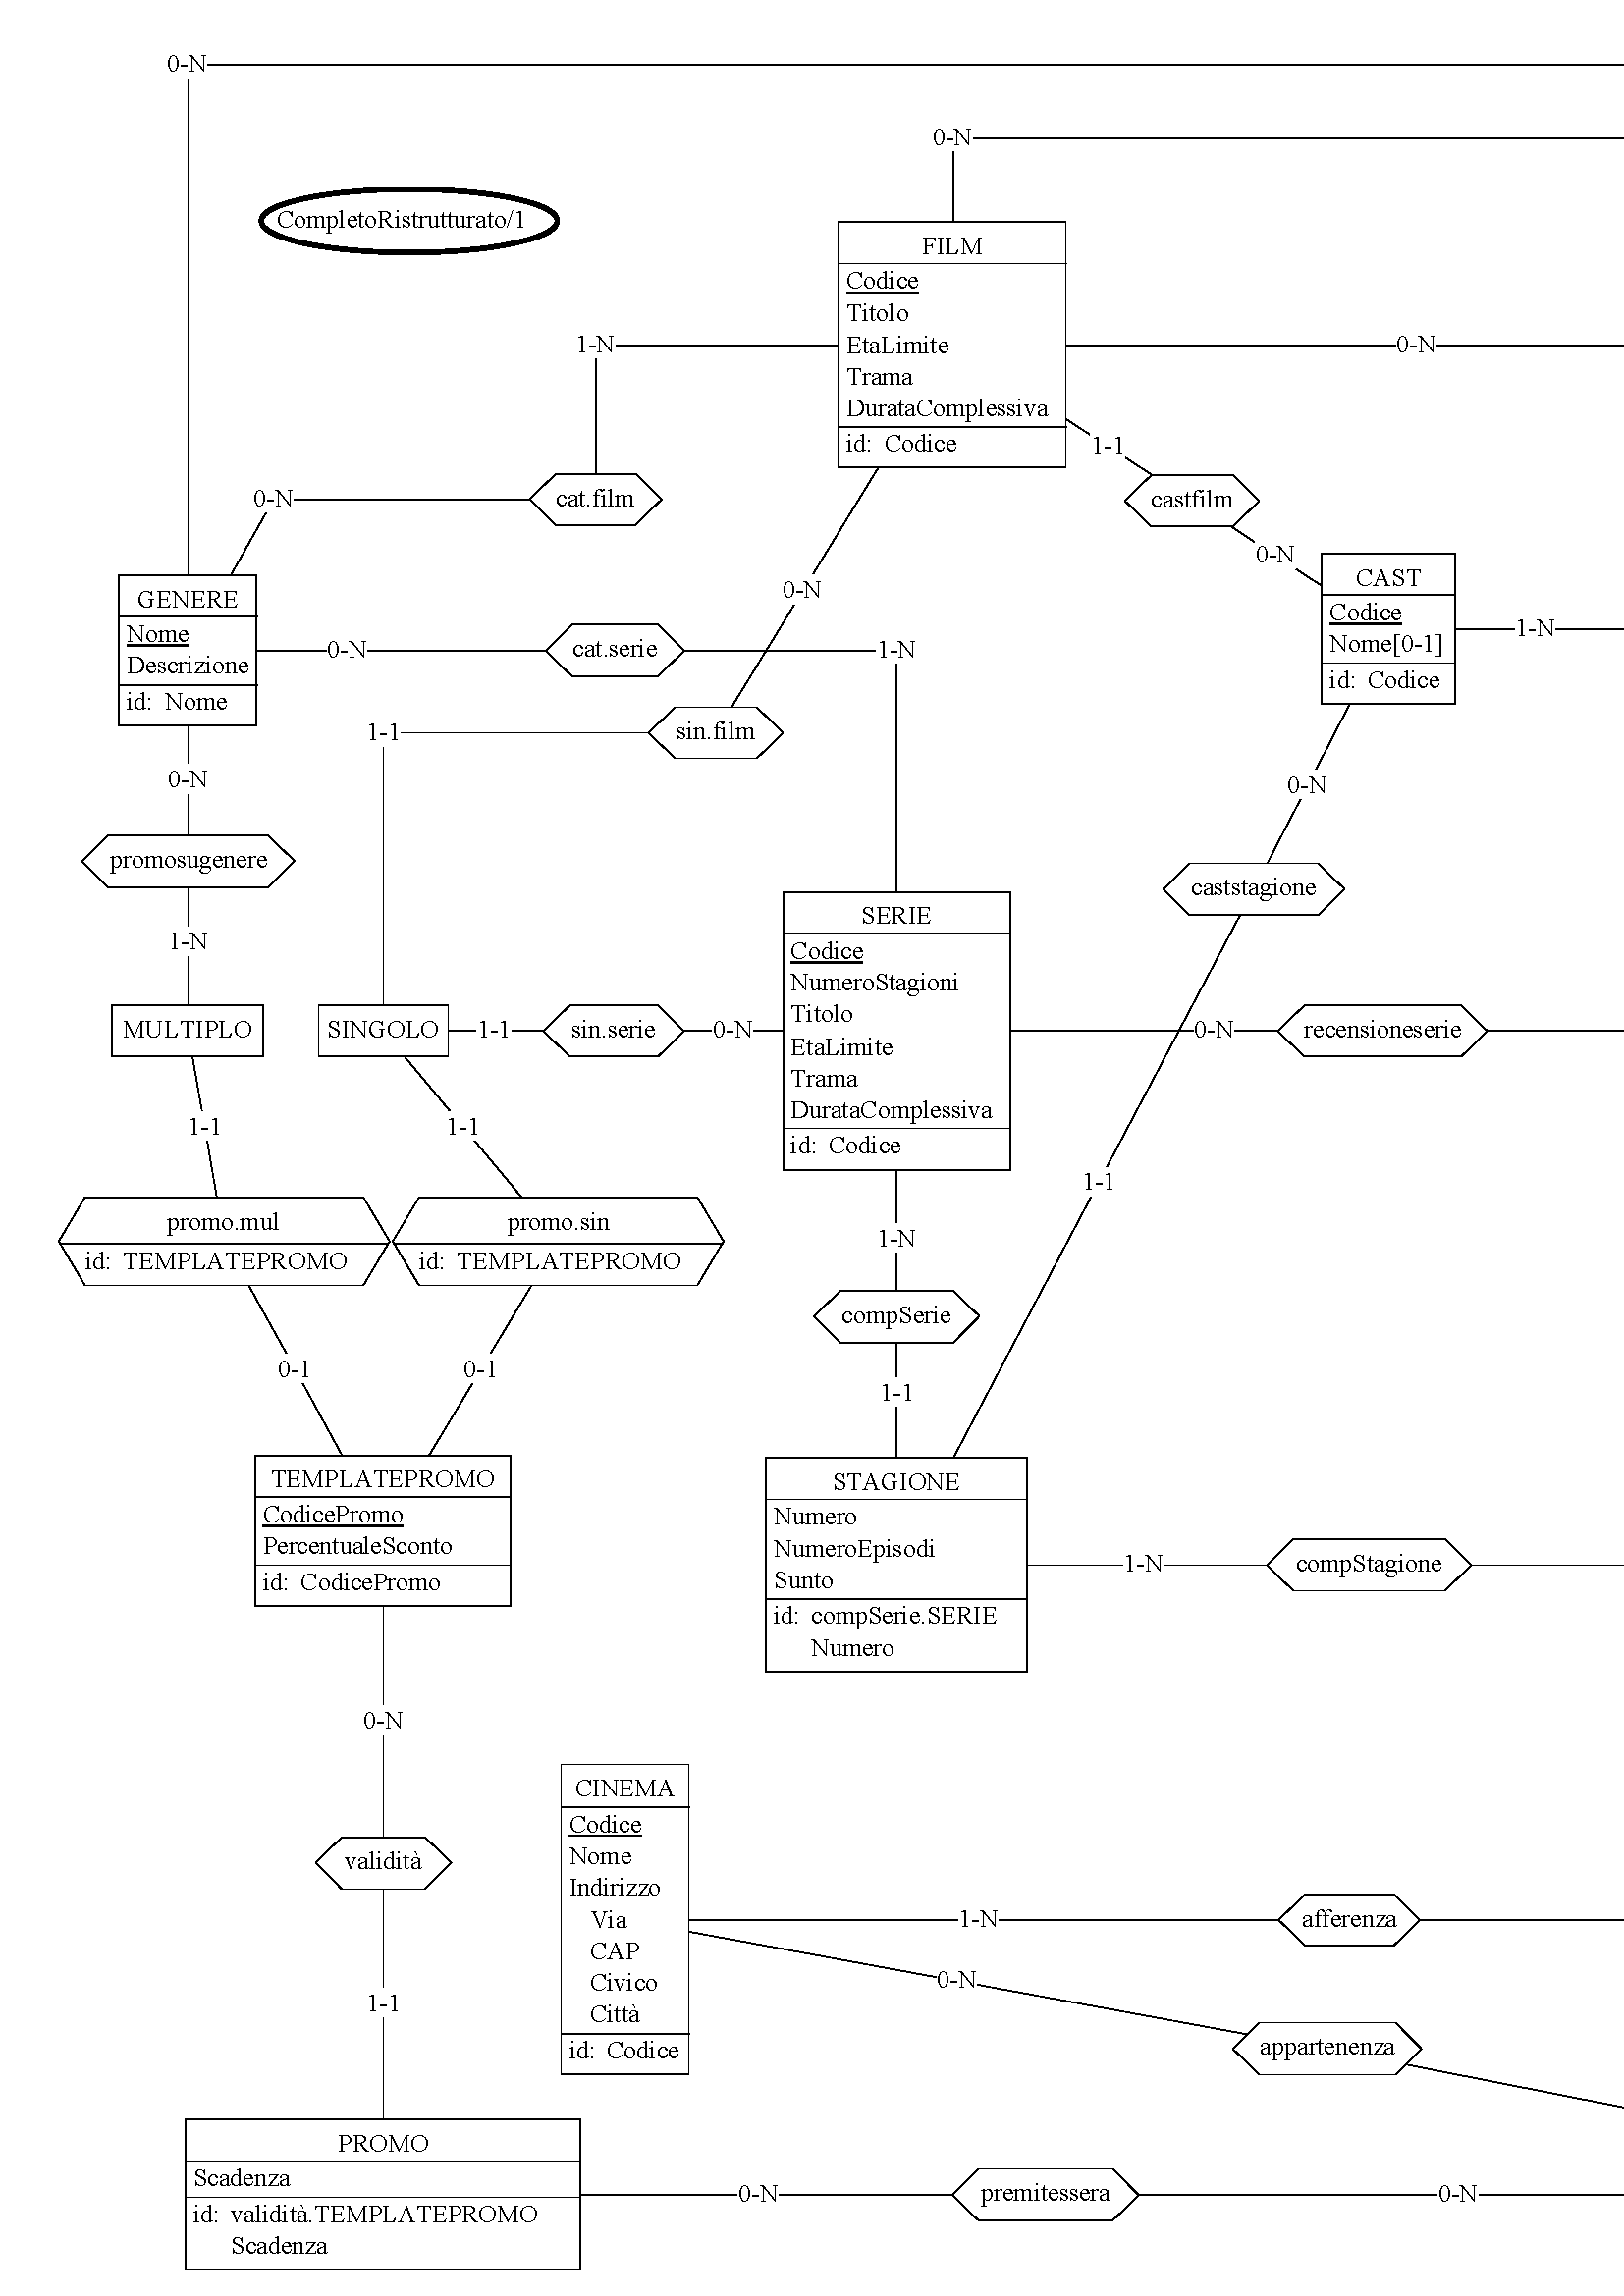
\includegraphics[width=450pt]{ER/ristrutturazione/ristcomp1.png}
	\caption{Schema ristrutturato completo \textbf{1/2}}
\end{figure}
\begin{figure}[H]
	\centering
	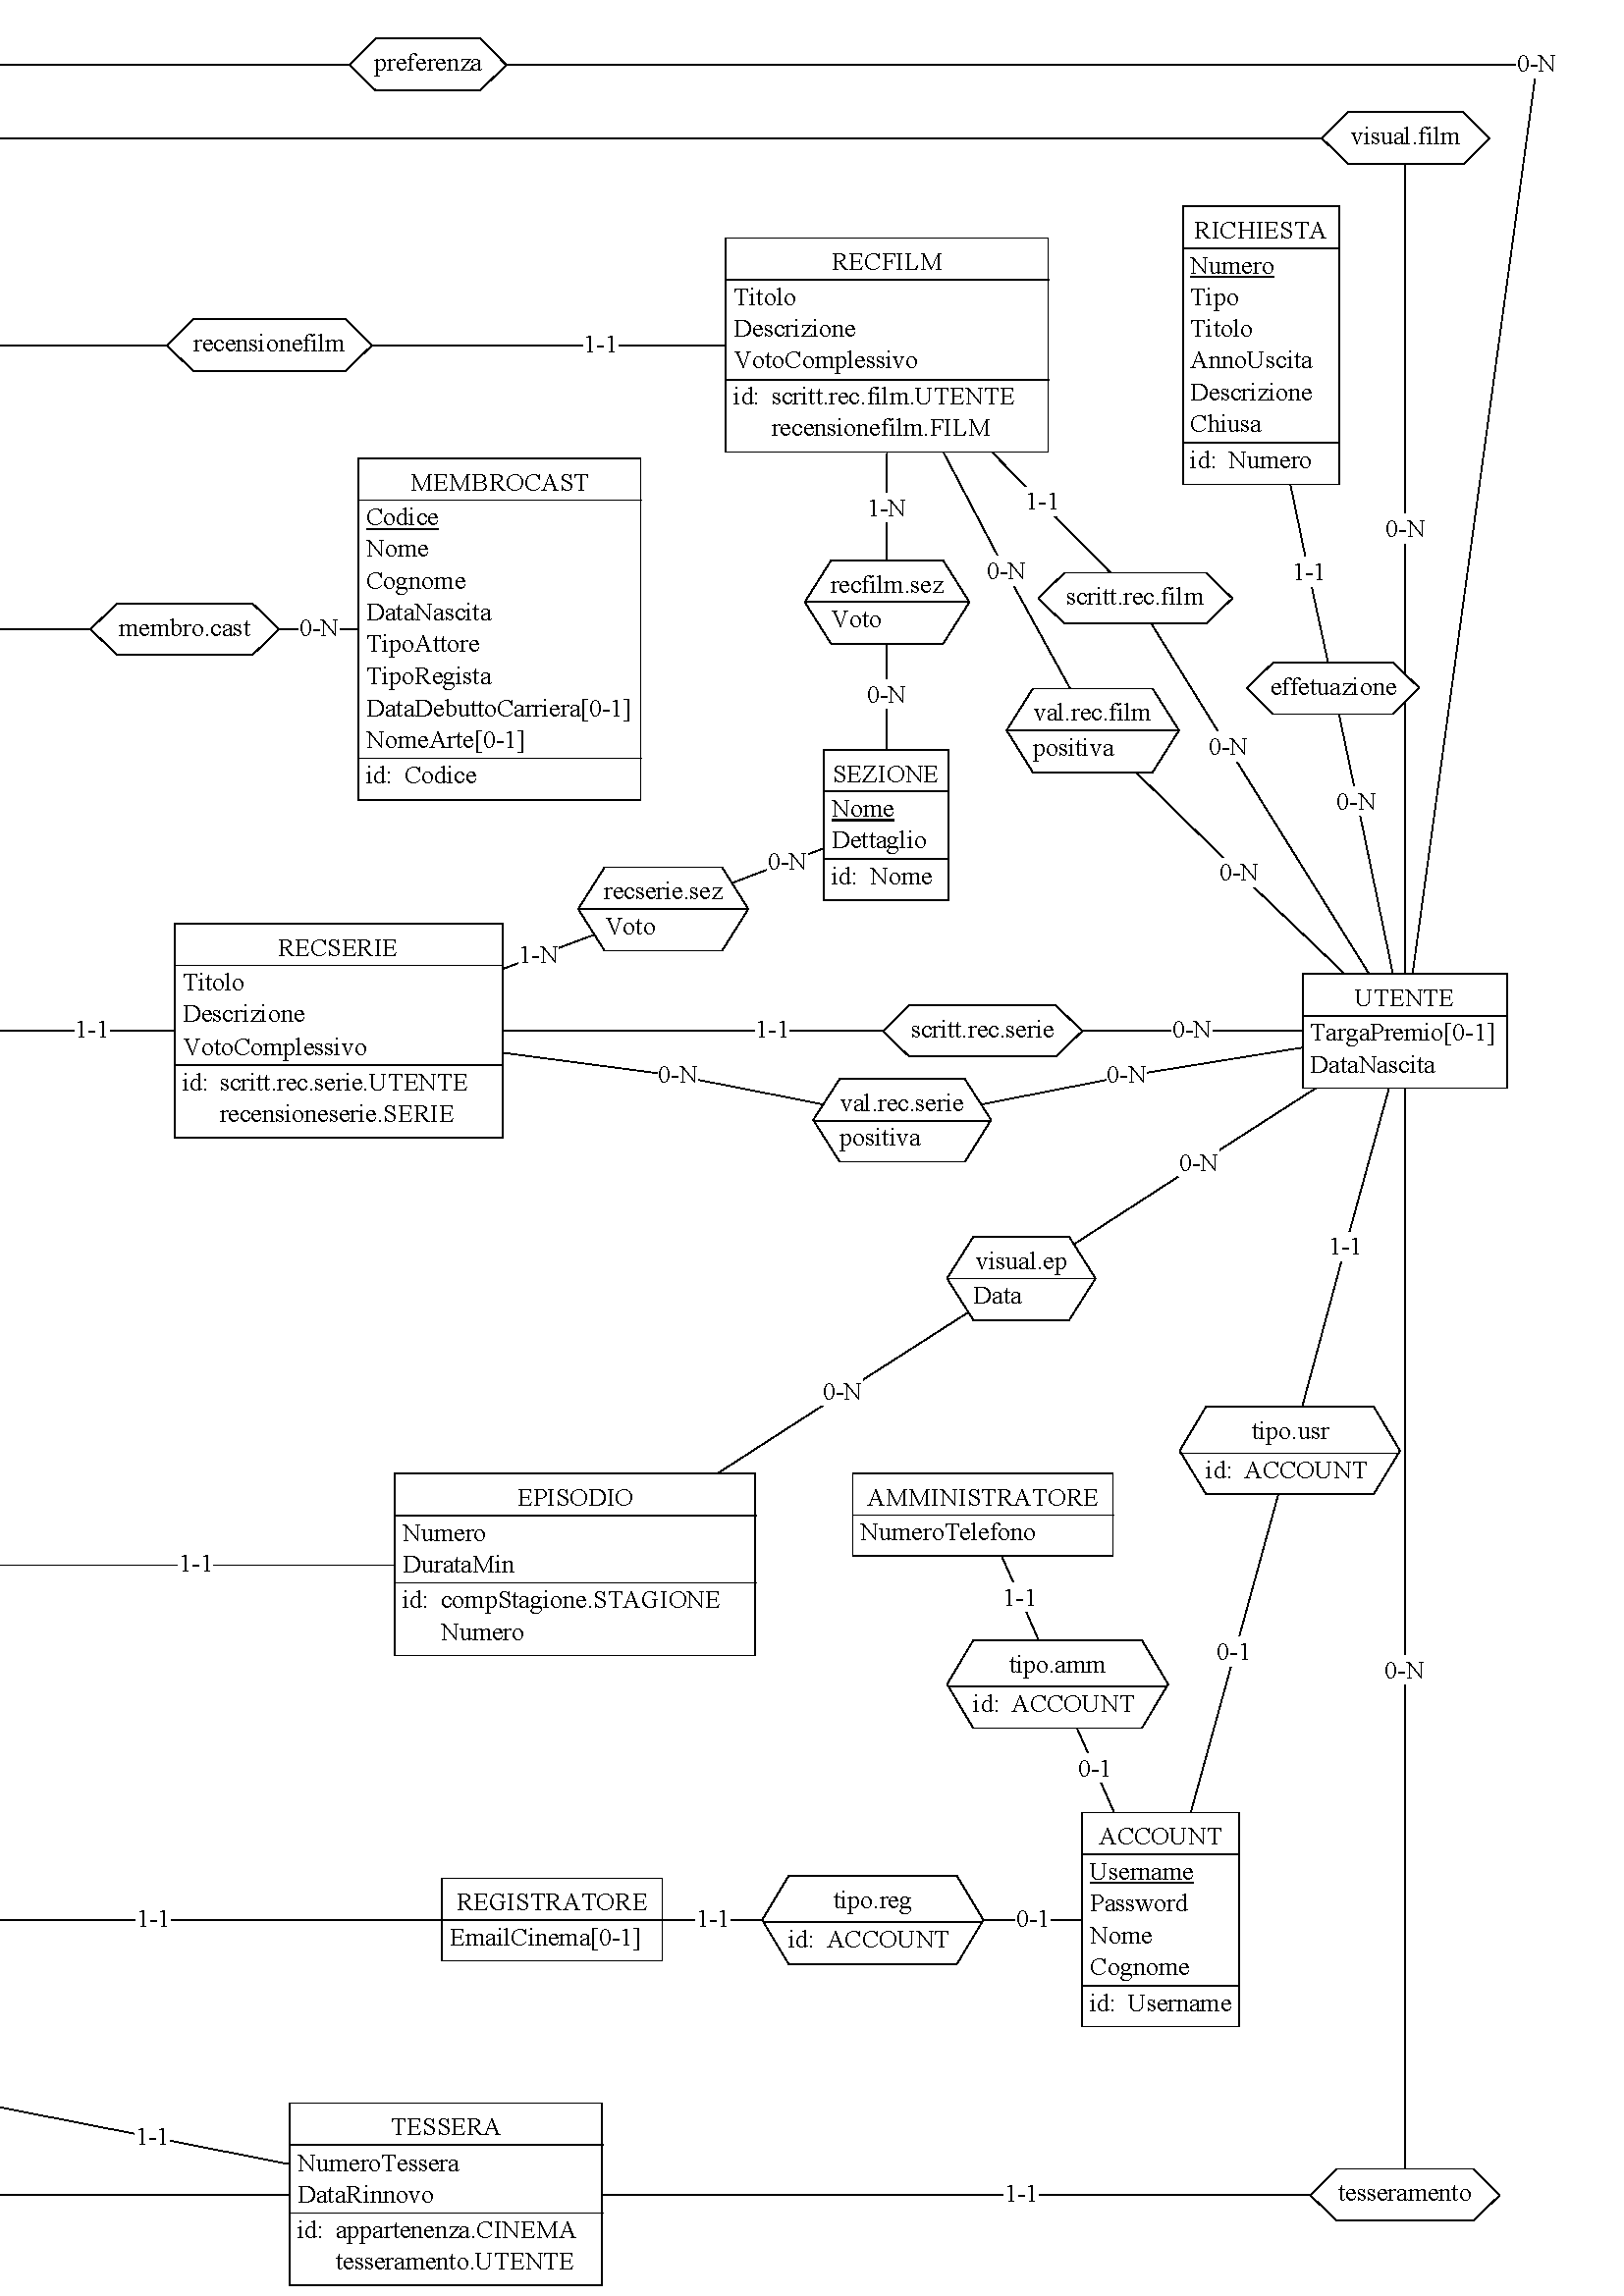
\includegraphics[width=450pt]{ER/ristrutturazione/ristcomp2.png}
	\caption{Schema ristrutturato completo \textbf{2/2}}
\end{figure}

\section{Schemi di navigazione e tabelle degli accessi - Operazioni Utente}
Questi schemi gestiscono il caso senza alcuna ridondanza introdotta, le ridondanze verranno discusse nella sezione successiva con riferimenti a questa per le tabelle degli accessi senza ridondanza.
\subsubsection{Registrazione di un nuovo utente (Op. 1)}
\begin{figure}[H]
	\centering
	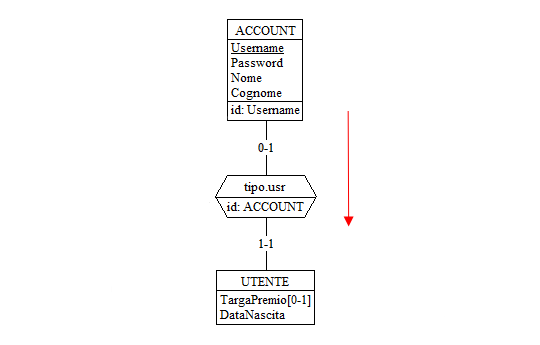
\includegraphics[width=450pt]{ER/navigazione/registrazioneutente.png}
	\caption{Schema di navigazione - registrazione nuovo utente}
\end{figure}
\begin{table}[H]
	\centering
	\begin{tabular}{|llll|}
		\hline
		\rowcolor[HTML]{CBCEFB}
		Concetto & Costrutto & Accesso & Tipo                             \\ \hline
		ACCOUNT  & E         & 1       & S                                \\ \hline
		UTENTE   & E         & 1       & S                                \\ \hline
		tipo.usr & R         & 1       & S                                \\ \hline
		\rowcolor[HTML]{CBCEFB}
		\multicolumn{4}{|l|}{\cellcolor[HTML]{FFCE93}\textbf{Totale}: 3S} \\ \hline
	\end{tabular}
\end{table}

\subsubsection{Accesso alla piattaforma di un utente (Op. 2.1)}
\begin{figure}[H]
	\centering
	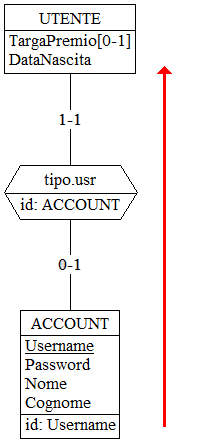
\includegraphics[width=200pt]{ER/navigazione/accessoutente.png}
	\caption{Schema di navigazione - Accesso utente}
\end{figure}
\begin{table}[H]
	\centering
	\begin{tabular}{|llll|}
		\hline
		\rowcolor[HTML]{CBCEFB}
		Concetto & Costrutto & Accesso & Tipo                             \\ \hline
		ACCOUNT  & E         & 1       & L                                \\ \hline
		UTENTE   & E         & 1       & L                                \\ \hline
		tipo.usr & R         & 1       & L                                \\ \hline
		\rowcolor[HTML]{CBCEFB}
		\multicolumn{4}{|l|}{\cellcolor[HTML]{FFCE93}\textbf{Totale}: 3L} \\ \hline
	\end{tabular}
\end{table}

\subsection{Accesso alla piattaforma di un amministratore (Op. 2.2)}
\begin{figure}[H]
	\centering
	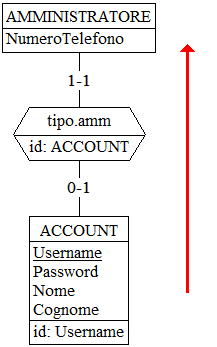
\includegraphics[width=250pt]{ER/navigazione/accessoamm.png}
	\caption{Schema di navigazione - Accesso amministratore}
\end{figure}
\begin{table}[H]
	\centering
	\begin{tabular}{|llll|}
		\hline
		\rowcolor[HTML]{CBCEFB}
		Concetto       & Costrutto & Accesso & Tipo                       \\ \hline
		ACCOUNT        & E         & 1       & L                          \\ \hline
		AMMINISTRATORE & E         & 1       & L                          \\ \hline
		tipo.amm       & R         & 1       & L                          \\ \hline
		\rowcolor[HTML]{CBCEFB}
		\multicolumn{4}{|l|}{\cellcolor[HTML]{FFCE93}\textbf{Totale}: 3L} \\ \hline
	\end{tabular}
\end{table}

\subsection{Accesso alla piattaforma di un registratore (Op. 2.3)}
\begin{figure}[H]
	\centering
	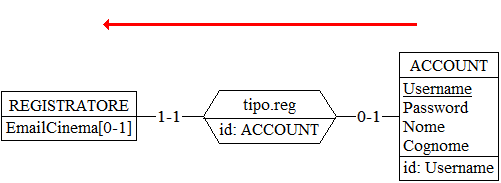
\includegraphics{ER/navigazione/accessoreg.png}
	\caption{Schema di navigazione - Accesso registratore}
\end{figure}
\begin{table}[H]
	\centering
	\begin{tabular}{|llll|}
		\hline
		\rowcolor[HTML]{CBCEFB}
		Concetto     & Costrutto & Accesso & Tipo                         \\ \hline
		ACCOUNT      & E         & 1       & L                            \\ \hline
		REGISTRATORE & E         & 1       & L                            \\ \hline
		tipo.reg     & R         & 1       & L                            \\ \hline
		\rowcolor[HTML]{CBCEFB}
		\multicolumn{4}{|l|}{\cellcolor[HTML]{FFCE93}\textbf{Totale}: 3L} \\ \hline
	\end{tabular}
\end{table}

\todo{Op. 3.*}

\subsection{Visualizzare tutto l'elenco dei film in base all'età di chi lo richiede (Op. 4.1)}
\begin{figure}[H]
	\centering
	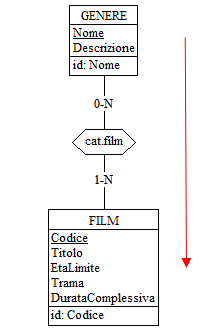
\includegraphics[width=300pt]{ER/navigazione/visualizzarefilm.png}
	\caption{Schema di navigazione - visualizzare elenco film}
\end{figure}
\begin{table}[H]
	\centering
	\begin{tabular}{|llll|}
		\hline
		\rowcolor[HTML]{CBCEFB}
		Concetto & Costrutto & Accesso & Tipo                                \\ \hline
		FILM     & E         & 9500    & L                                   \\ \hline
		UTENTE   & E         & 1       & L                                   \\ \hline
		ACCOUNT  & E         & 1       & L                                   \\ \hline
		tipo.usr & R         & 1       & L                                   \\ \hline
		\rowcolor[HTML]{CBCEFB}
		\multicolumn{4}{|l|}{\cellcolor[HTML]{FFCE93}\textbf{Totale}: 9503L} \\ \hline
	\end{tabular}
\end{table}

\subsection{Visualizzare l’elenco dei film in base ad un’età scelta. (Op. 4.2)}
In media gli utenti che richiedono la visualizzazione dei film sono principalmente adulti, quindi la maggior parte visualizzerà tutti i film (9500).
\begin{figure}[H]
	\centering
	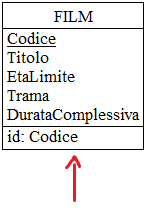
\includegraphics{ER/navigazione/visualizzarefilm2.png}
	\caption{Schema di navigazione - Visualizzare elenco film in base all'età}
\end{figure}
\begin{table}[H]
	\centering
	\begin{tabular}{|llll|}
		\hline
		\rowcolor[HTML]{CBCEFB}
		Concetto & Costrutto & Accesso & Tipo                                \\ \hline
		FILM     & E         & 9500    & L                                   \\ \hline
		\rowcolor[HTML]{CBCEFB}
		\multicolumn{4}{|l|}{\cellcolor[HTML]{FFCE93}\textbf{Totale}: 9500L} \\ \hline
	\end{tabular}
\end{table}

\subsection{Visualizzare l’elenco delle serie TV con la relativa durata complessiva e il numero di stagioni ed episodi complessivo, in base all’età di chi lo richiede. (Op. 4.3)} \label{ss:op43}
\begin{figure}[H]
	\centering
	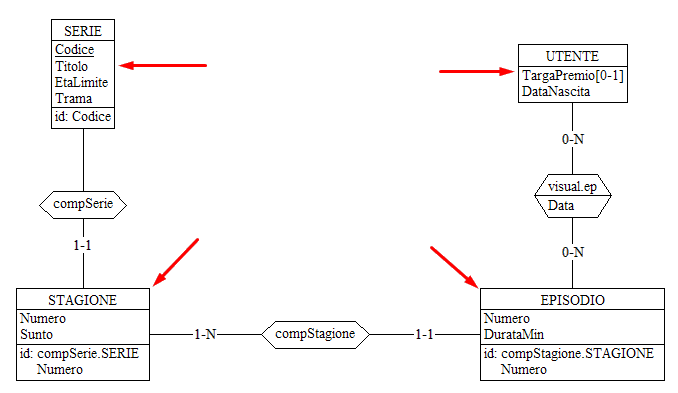
\includegraphics[width=1.2\linewidth]{ER/navigazione/elencoserietv.png}
	\caption{}
	\label{fig:elencoserietv}
\end{figure}
\begin{table}[H]
	\centering
	\begin{tabular}{|llll|}
		\hline
		\rowcolor[HTML]{CBCEFB}
		Concetto & Costrutto & Accesso & Tipo                                   \\ \hline
		UTENTE   & E         & 1       & L                                      \\ \hline
		SERIE    & E         & 2500    & L                                      \\ \hline
		STAGIONE & E         & 10.000  & L                                      \\ \hline
		EPISODIO & E         & 400.000 & L                                      \\ \hline
		\rowcolor[HTML]{CBCEFB}
		\multicolumn{4}{|l|}{\cellcolor[HTML]{FFCE93}\textbf{Totale}: 412.501L} \\ \hline
	\end{tabular}
\end{table}

\subsection{Visualizzare le informazioni riguardanti una serie TV, comprese tutte le stagioni e tutti gli episodi. (Op. 4.4)} \label{ss:op44}
\begin{figure}[H]
	\centering
	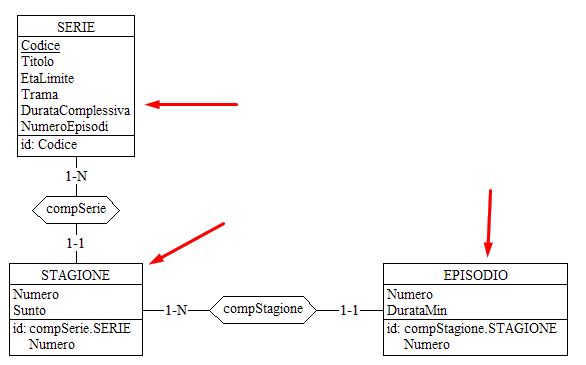
\includegraphics[width=1.2\linewidth]{ER/navigazione/infoserietv.png}
	\caption{Schema di navigazione - Visualizzare elenco serie tv in base all'età}
\end{figure}
Per ogni serie vi sono in media $\frac{10000}{2500} = 4$ stagioni, che si compongono ciascuna di $\frac{400000}{10000 * 4} = 10$ episodi complessivi.
\begin{table}[H]
	\centering
	\begin{tabular}{|llll|}
		\hline
		\rowcolor[HTML]{CBCEFB}
		Concetto & Costrutto & Accesso & Tipo                              \\ \hline
		SERIE    & E         & 1       & L                                 \\ \hline
		STAGIONE & E         & 4       & L                                 \\ \hline
		EPISODIO & E         & 40      & L                                 \\ \hline
		\rowcolor[HTML]{CBCEFB}
		\multicolumn{4}{|l|}{\cellcolor[HTML]{FFCE93}\textbf{Totale}: 45L} \\ \hline
	\end{tabular}
\end{table}

\subsection{Aggiunta di una nuova stagione per una specifica serie TV. (Op. 4.5)} \label{ss:op45}
Per questa Operazione, é necessaria la lettura della serie per poter aggiungere una nuova stagione e legarla tramite l'associazione compSerie. Inoltre, va aggiunto un nuovo episodio alla stagione aggiunta, essendo la cardinalitá minima obbligatoria che lega episodio a stagione.
\begin{figure}[H]
	\centering
	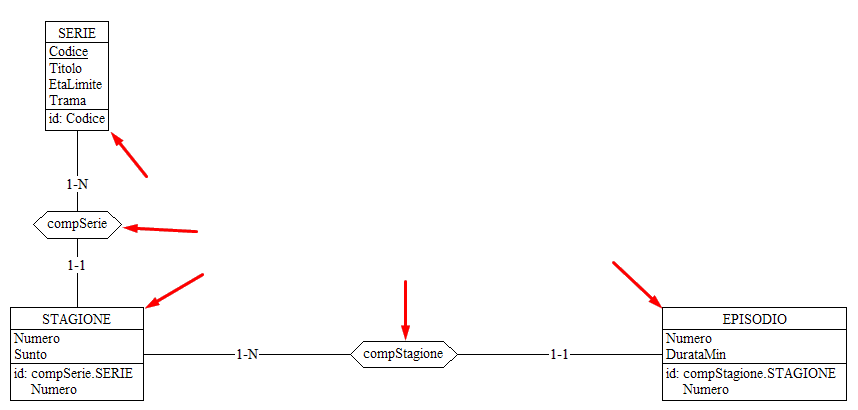
\includegraphics[width=1.2\linewidth]{ER/navigazione/aggiuntastagione.png}
	\caption{Schema di navigazione - Aggiunta di nuova stagione per serie TV}
\end{figure}
\begin{table}[H]
	\centering
	\begin{tabular}{|llll|}
		\hline
		\rowcolor[HTML]{CBCEFB}
		Concetto 		& Costrutto & Accesso 	& Tipo                              \\ \hline
		SERIE   		& E     	& 1       	& L                                 \\ \hline
		STAGIONE 		& E         & 1       	& S                                 \\ \hline
		EPISODIO 		& E         & 1       	& S                                 \\ \hline
		compSerie 		& R         & 1       	& S                                 \\ \hline
		compStagione	& R         & 1       	& S                                 \\ \hline
		\rowcolor[HTML]{CBCEFB}
		\multicolumn{4}{|l|}{\cellcolor[HTML]{FFCE93}\textbf{Totale}: 1L+4S} \\ \hline
	\end{tabular}
\end{table}

\subsection{Aggiunta di un nuovo episodio per una specifica stagione di una serie TV. (Op. 4.6)} \label{ss:op46}
\begin{figure}[H]
	\centering
	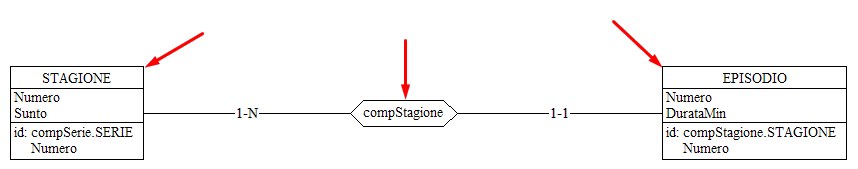
\includegraphics[width=1.2\linewidth]{ER/navigazione/aggiuntaepisodio.png}
	\caption{Schema di navigazione - Aggiunta di nuovo episodio per stagione serie TV.}
\end{figure}
\begin{table}[H]
	\centering
	\begin{tabular}{|llll|}
		\hline
		\rowcolor[HTML]{CBCEFB}
		Concetto 		& Costrutto & Accesso 	& Tipo                              \\ \hline
		STAGIONE 		& E         & 1       	& L                                 \\ \hline
		EPISODIO 		& E         & 1       	& S                                 \\ \hline
		compStagione	& R         & 1       	& S                                 \\ \hline
		\rowcolor[HTML]{CBCEFB}
		\multicolumn{4}{|l|}{\cellcolor[HTML]{FFCE93}\textbf{Totale}: 1L+2S} \\ \hline
	\end{tabular}
\end{table}

\subsection{Contrassegnare come ”visualizzato” un film (Op. 5.1)} \label{ss:op51}
\begin{figure}[H]
	\centering
	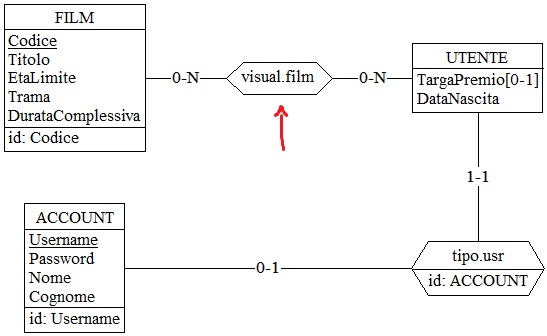
\includegraphics[width=300pt]{ER/navigazione/visualizzatofilm.png}
	\caption{Schema di navigazione - Contrassegnare un film "visualizzato"}
\end{figure}
\begin{table}[H]
	\centering
	\begin{tabular}{|llll|}
		\hline
		\rowcolor[HTML]{CBCEFB}
		Concetto            & Costrutto & Accesso & Tipo                  \\ \hline
		visualizzazionefilm & R         & 1       & S                     \\ \hline
		\rowcolor[HTML]{CBCEFB}
		\multicolumn{4}{|l|}{\cellcolor[HTML]{FFCE93}\textbf{Totale}: 1S} \\ \hline
	\end{tabular}
\end{table}

\subsection{Contrassegnare come ”visualizzato” un episodio di una serie (Op. 5.2)} \label{ss:op52}
\begin{figure}[H]
	\centering
	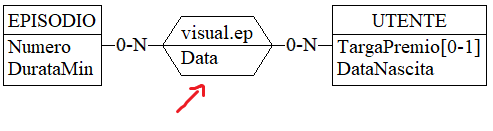
\includegraphics{ER/navigazione/visualizzatoep.png}
	\caption{Schema di navigazione - Contrassegnare un episodio di una serie "visualizzato"}
\end{figure}
\begin{table}[H]
	\centering
	\begin{tabular}{|llll|}
		\hline
		\rowcolor[HTML]{CBCEFB}
		Concetto          & Costrutto & Accesso & Tipo                    \\ \hline
		visualizzazioneep & R         & 1       & S                       \\ \hline
		\rowcolor[HTML]{CBCEFB}
		\multicolumn{4}{|l|}{\cellcolor[HTML]{FFCE93}\textbf{Totale}: 1S} \\ \hline
	\end{tabular}
\end{table}

\subsection{Recensire un film (Op. 6)}
\begin{figure}[H]
	\centering
	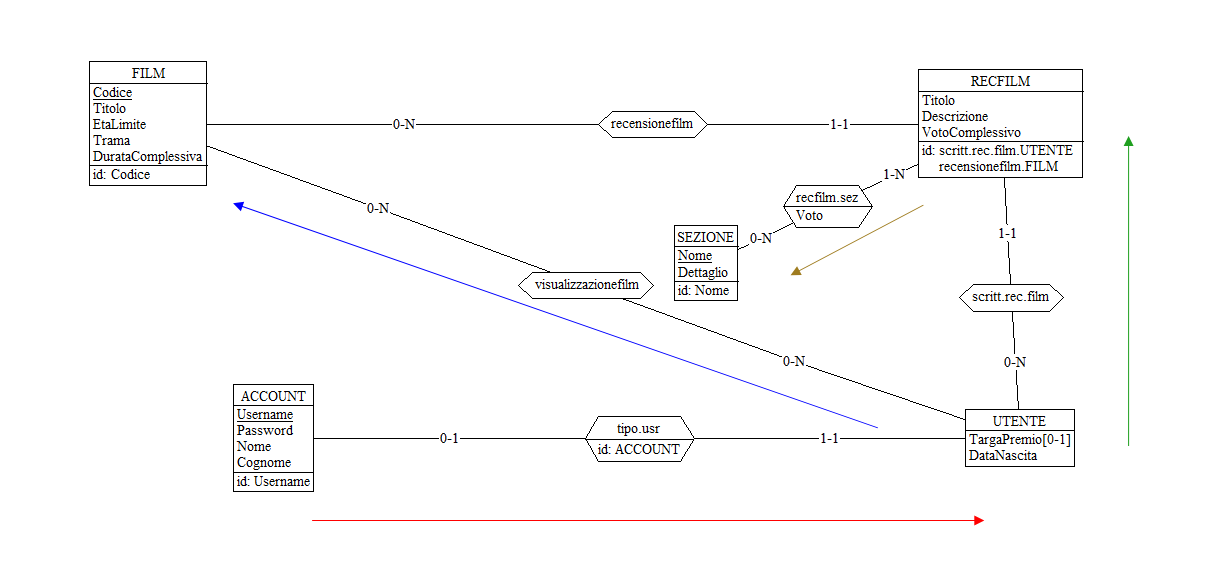
\includegraphics[width=450pt]{ER/navigazione/recensionefilm.png}
	\caption{Schema di navigazione - recensire un film}
\end{figure}
\begin{table}[H]
	\centering
	\begin{tabular}{|llll|}
		\hline
		\rowcolor[HTML]{CBCEFB}
		Concetto        & Costrutto & Accesso & Tipo                            \\ \hline
		SEZIONE         & E         & 5       & S                               \\ \hline
		RECFILM         & E         & 1       & S                               \\ \hline
		visual.film     & R         & 1       & L                               \\ \hline
		recfilm.sez     & R         & 5       & S                               \\ \hline
		scritt.rec.film & R         & 1       & S                               \\ \hline
		\rowcolor[HTML]{CBCEFB}
		\multicolumn{4}{|l|}{\cellcolor[HTML]{FFCE93}\textbf{Totale}: 1L + 12S} \\ \hline
	\end{tabular}
\end{table}

\subsection{Visualizzare le recensioni di un film (Op. 7.1)}
Considerando la tabella dei volumi (sez: \ref{s:volumes}), un film ha in media $\frac{950000}{9500} = 100$ recensioni.
\begin{figure}[H]
	\centering
	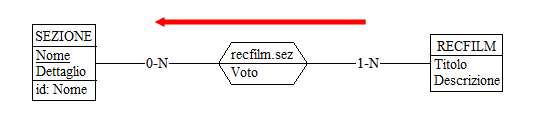
\includegraphics[width=450pt]{ER/navigazione/visualrecensionifilm.png}
	\caption{Schema di navigazione - Visualizzare le recensioni di un film}
\end{figure}
\begin{table}[H]
	\centering
	\begin{tabular}{|llll|}
		\hline
		\rowcolor[HTML]{CBCEFB}
		Concetto    & Costrutto & Accesso & Tipo                             \\ \hline
		RECFILM     & E         & 100     & L                                \\ \hline
		recfilm.sez & R         & 500     & L                                \\ \hline
		\rowcolor[HTML]{CBCEFB}
		\multicolumn{4}{|l|}{\cellcolor[HTML]{FFCE93}\textbf{Totale}: 600L} \\ \hline
	\end{tabular}
\end{table}

\subsection{Dare una valutazione di utilità ad una recensione di un altro utente su un film. (Op. 7.2)}
\begin{figure}[H]
	\centering
	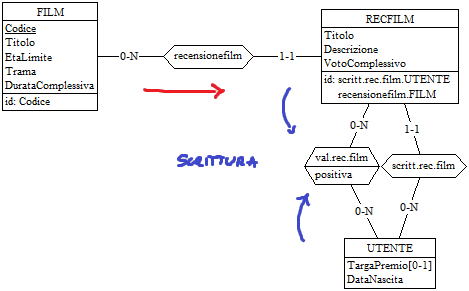
\includegraphics[width=450pt]{ER/navigazione/valutazionerecfilm.png}
	\caption{Schema di navigazione - Dare una valutazione di utilità ad una recensione di un altro utente su un film.}
\end{figure}
\begin{table}[H]
	\centering
	\begin{tabular}{|llll|}
		\hline
		\rowcolor[HTML]{CBCEFB}
		Concetto     & Costrutto & Accesso & Tipo                         \\ \hline
		val.rec.film & R         & 1       & S                            \\ \hline
		\rowcolor[HTML]{CBCEFB}
		\multicolumn{4}{|l|}{\cellcolor[HTML]{FFCE93}\textbf{Totale}: 1S} \\ \hline
	\end{tabular}
\end{table}

\subsection{Dare una valutazione di utilità ad una recensione di un altro utente su una serie tv. (Op. 7.3)}
\begin{figure}[H]
	\centering
	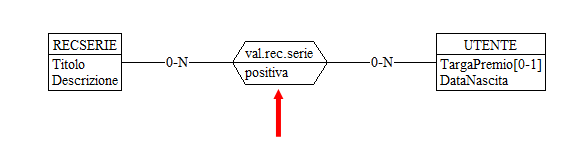
\includegraphics[width=450pt]{ER/navigazione/valutazionerecserie.png}
	\caption{Schema di navigazione - Dare una valutazione di utilità ad una recensione di un altro utente su una serie.}
\end{figure}
\begin{table}[H]
	\centering
	\begin{tabular}{|llll|}
		\hline
		\rowcolor[HTML]{CBCEFB}
		Concetto      & Costrutto & Accesso & Tipo                        \\ \hline
		val.rec.serie & R         & 1       & S                           \\ \hline
		\rowcolor[HTML]{CBCEFB}
		\multicolumn{4}{|l|}{\cellcolor[HTML]{FFCE93}\textbf{Totale}: 1S} \\ \hline
	\end{tabular}
\end{table}

\subsection{Visualizzare le recensioni di una singola serie (Op. 7.4)}
Considerando la tabella dei volumi (sez: \ref{s:volumes}), una serie ha in media $\frac{250000}{2500} = 100$ recensioni e ciascuna recensione è articolata nel caso con maggior volume in tutte e 5 le sezioni.
\begin{figure}[H]
	\centering
	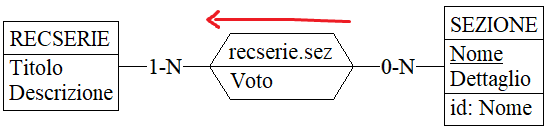
\includegraphics{ER/navigazione/visualrecserie.png}
	\caption{Schema di navigazione - Visualizzare le recensioni di una serie.}
\end{figure}
\begin{table}[H]
	\centering
	\begin{tabular}{|llll|}
		\hline
		\rowcolor[HTML]{CBCEFB}
		Concetto     & Costrutto & Accesso & Tipo                            \\ \hline
		RECSERIE     & E         & 100     & L                               \\ \hline
		recserie.sez & R         & 500     & L                               \\ \hline
		\rowcolor[HTML]{CBCEFB}
		\multicolumn{4}{|l|}{\cellcolor[HTML]{FFCE93}\textbf{Totale}: 600L} \\ \hline
	\end{tabular}
\end{table}

\subsection{Aggiornare il voto di una sezione di una recensione (Op. 7.5)}
\begin{figure}[H]
	\centering
	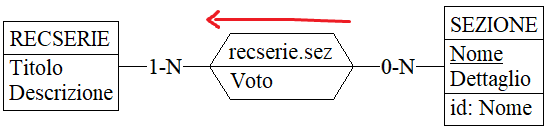
\includegraphics{ER/navigazione/visualrecserie.png}
	\caption{Schema di navigazione - Aggiornare una sezione di una recensione.}
\end{figure}
\begin{table}[H]
	\centering
	\begin{tabular}{|llll|}
		\hline
		\rowcolor[HTML]{CBCEFB}
		Concetto     & Costrutto & Accesso & Tipo                            \\ \hline
		recserie.sez     & R         & 1     & S                               \\ \hline
		recserie.sez & R         & 1     & L                               \\ \hline
		\rowcolor[HTML]{CBCEFB}
		\multicolumn{4}{|l|}{\cellcolor[HTML]{FFCE93}\textbf{Totale}: 1S + 1L} \\ \hline
	\end{tabular}
\end{table}

\subsection{Ottenere una classifica dei generi più visualizzati (Op. 8.1)} \label{ss:op81}
Per questa operazione consideriamo che: Ci sono in tutto $13$ generi che vengono memorizzati, questi andranno letti tutti dato che è una classifica. Ci interessano inoltre le relazioni \textit{visualizzazioneep} (Visualizzazione Episodio) e \textit{visualizzazionefilm} (Visualizzazione Film), complessivamente, un utente visualizza in media $\frac{350000}{9960} \approx 35$ film, avendo i film visualizzati, possiamo calcolare quanti generi sono stati visualizzati in media: $\frac{23500}{9500} \approx 2$, ricapitolando i volumi per le visualizzazioni dei film in media sono:
\begin{itemize}
	\item 35 su visualizzazionefilm (per utente).
	\item 2 su cat.film (per film visualizzato).
	\item 13 su genere.
\end{itemize}
Per le serie il ragionamento ha qualche variazione, in particolare per ogni serie vi sono in media \\ $\frac{10000}{2500} = 4$ stagioni,\\ che si compongono ciascuna di \\ $\frac{400000}{10000 * 4} = 10$ episodi complessivi.\\ In media un utente visualizza $\frac{1400000}{9960} \approx 146$ episodi in tutto, quindi si può constatare che un utente visualizza $\frac{146}{10} \approx 15$ stagioni complessive, e di conseguenza $\frac{4}{15} \approx 0,3$ serie.\\
Otteniamo:
\begin{itemize}
	\item 146 su visualizzazioneep (per utente)
	\item 4 su STAGIONE (per utente)
	\item 0,3 su SERIE (per utente)
	\item 2 su cat.serie (per serie visualizzata da un utente)
\end{itemize}
\begin{figure}[H]
	\centering
	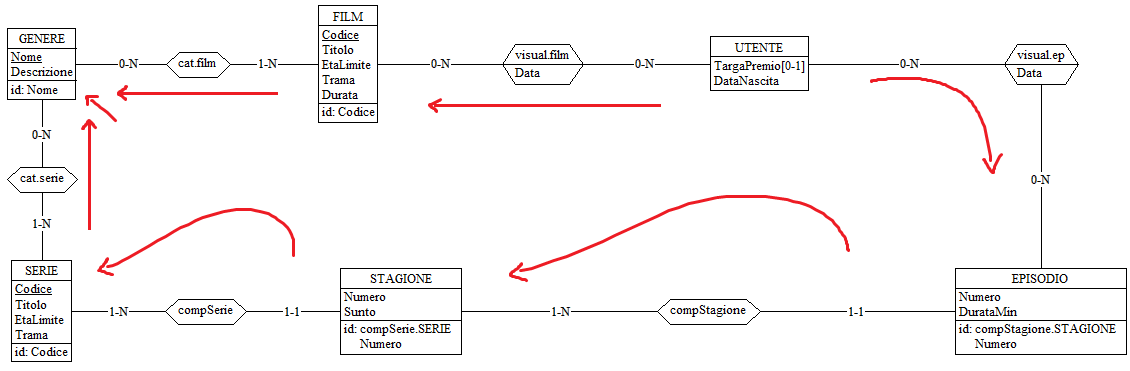
\includegraphics[width=450pt]{ER/navigazione/classificageneri.png}
	\caption{Schema di navigazione - visualizzare classifica dei generi più visualizzati}
\end{figure}
\begin{table}[H]
	\centering
	\begin{tabular}{|llll|}
		\hline
		\rowcolor[HTML]{CBCEFB}
		Concetto            & Costrutto & Accesso   & Tipo                         \\ \hline
		GENERE              & E         & 13        & L                            \\ \hline
		STAGIONE            & E         & 39.840    & L                            \\ \hline
		SERIE               & E         & 2.988     & L                            \\ \hline
		visualizzazioneep   & R         & 1.454.160 & L                            \\ \hline
		cat.serie           & R         & 5.976     & L                            \\ \hline
		visualizzazionefilm & R         & 348.600   & L                            \\ \hline
		cat.film            & R         & 697.200   & L                            \\ \hline
		\rowcolor[HTML]{CBCEFB}
		\multicolumn{4}{|l|}{\cellcolor[HTML]{FFCE93}\textbf{Totale}: 2.548.776 L} \\ \hline
	\end{tabular}
\end{table}

\subsection{Visualizzare una classifica dei registi più apprezzati (Op. 8.2)}
\begin{figure}[H]
	\centering
	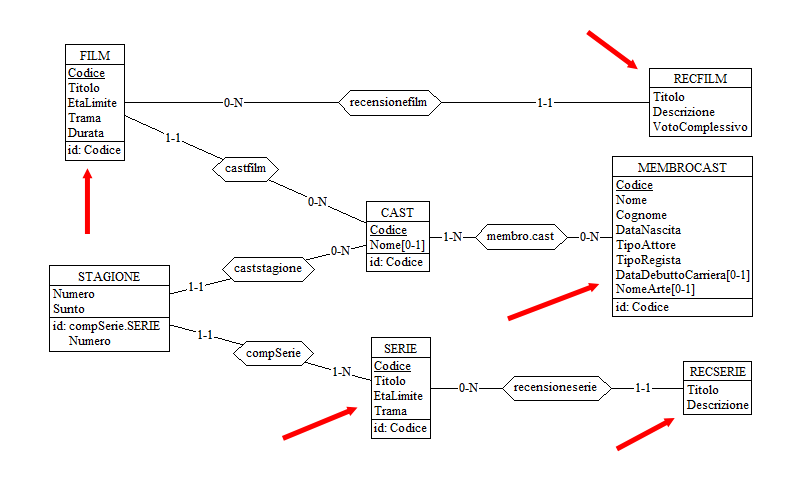
\includegraphics[width=450pt]{ER/navigazione/classificaregisti.png}
	\caption{Schema di navigazione - visualizzare classifica dei registi più apprezzati}
\end{figure}
Questa operazione richiede di tenere conto del fatto che le recensioni fornite per un film o una serie TV sono attribuite a loro volta al regista, poiché è univoco per ciascun multimedia. Pertanto, è essenziale esaminare ogni recensione sia per i film che per le serie TV, così come i relativi prodotti multimediali e i registi che li hanno realizzati.
\begin{table}[H]
	\centering
	\begin{tabular}{|llll|}
		\hline
		\rowcolor[HTML]{CBCEFB}
		Concetto   & Costrutto & Accesso & Tipo                                    \\ \hline
		MEMBROCAST & E         & 600     & L                                       \\ \hline
		RECFILM    & E         & 950.000 & L                                       \\ \hline
		RECSERIE   & E         & 250.000 & L                                       \\ \hline
		\rowcolor[HTML]{CBCEFB}
		\multicolumn{4}{|l|}{\cellcolor[HTML]{FFCE93}\textbf{Totale}: 1.200.600 L} \\ \hline
	\end{tabular}
\end{table}

\section{Schemi di navigazione e tabelle degli accessi - Operazioni Amministratore}
\subsubsection{Visualizzare una classifica degli utenti con la media valutazioni di utilità peggiore (Op. 9.1)}
Per questa operazione bisogna valutare ogni utente e verificare ogni singola valutazione per le sue recensioni scritte. In media un utente scrive $\frac{1200000}{9960} \approx 120$ recensioni(in particolare $\frac{950000}{9960} \approx 95$ recensioni per i film e $\frac{250000}{9960} \approx 25$ recensioni per le serie tv). \\
Ciascuna recensione per un film riceve $\frac{950000}{115000} \approx 8$ valutazioni mentre per quanto riguarda le recensioni sulle serie tv ciascuna riceve $\frac{250000}{115000} \approx 2$ valutazioni. \\
Quindi complessivamente avremo $95 * 8 = 760$ valutazioni nelle recensioni per i film e $25 * 2 = 50$ valutazioni nelle recensioni per le serie tv che ha svolto un utente, per questo il tutto va moltiplicato per il numero di utenti.

\begin{figure}[H]
	\centering
	\includegraphics[width=450pt]{ER/navigazione/classificautilitápeggiore.png}
	\caption{Schema di navigazione - visualizzare classifica degli utenti con la media valutazioni di utilità peggiore}
\end{figure}
\begin{table}[H]
	\centering
	\begin{tabular}{|llll|}
		\hline
		\rowcolor[HTML]{CBCEFB}
		Concetto      & Costrutto & Accesso   & Tipo                               \\ \hline
		UTENTE        & E         & 9960      & L                                  \\ \hline
		val.rec.film  & R         & 7.569.600 & L                                  \\ \hline
		val.rec.serie & R         & 498.000   & L                                  \\ \hline
		\rowcolor[HTML]{CBCEFB}
		\multicolumn{4}{|l|}{\cellcolor[HTML]{FFCE93}\textbf{Totale}: 8.077.560 L} \\ \hline
	\end{tabular}
\end{table}

\subsubsection{Visualizzare una classifica degli utenti con la media valutazioni di utilità migliori (Op. 9.2)}
Per questa operazione il ragionamento è analogo a quella precedente(Op. 9.1).
\begin{figure}[H]
	\centering
	\includegraphics[width=450pt]{ER/navigazione/classificautilitámigliore.png}
	\caption{Schema di navigazione - visualizzare classifica degli utenti con la media valutazioni di utilità migliori}
\end{figure}
\begin{table}[H]
	\centering
	\begin{tabular}{|llll|}
		\hline
		\rowcolor[HTML]{CBCEFB}
		Concetto      & Costrutto & Accesso   & Tipo                               \\ \hline
		UTENTE        & E         & 9960      & L                                  \\ \hline
		val.rec.film  & R         & 7.569.600 & L                                  \\ \hline
		val.rec.serie & R         & 498.000   & L                                  \\ \hline
		\rowcolor[HTML]{CBCEFB}
		\multicolumn{4}{|l|}{\cellcolor[HTML]{FFCE93}\textbf{Totale}: 8.077.560 L} \\ \hline
	\end{tabular}
\end{table}

\subsubsection{Assegnamento in blocco di promozioni ai primi 5 utenti tesserati con la media valutazioni di utilità migliori (Op. 10)}
\begin{figure}[H]
	\centering
	
\includegraphics[width=450pt]{ER/navigazione/couponutentimigliori.png}
	\caption{Schema di navigazione - Operazione 10}
\end{figure}
\begin{table}[H]
	\centering
	\begin{tabular}{|llll|}
		\hline
		\rowcolor[HTML]{CBCEFB}
		Concetto     & Costrutto & Accesso & Tipo                         \\ \hline
		premitessera & R         & 5       & S                            \\ \hline
		\rowcolor[HTML]{CBCEFB}
		\multicolumn{4}{|l|}{\cellcolor[HTML]{FFCE93}\textbf{Totale}: 5S} \\ \hline
	\end{tabular}
\end{table}


\subsubsection{Aggiunta di un nuovo film alla piattaforma (Op. 11.1)}
\begin{figure}[H]
	\centering
	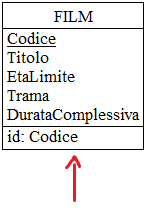
\includegraphics[width=150pt]{ER/navigazione/aggiuntafilm.png}
	\caption{Schema di navigazione - aggiunta nuovo film alla piattaforma}
\end{figure}
\begin{table}[H]
	\centering
	\begin{tabular}{|llll|}
		\hline
		\rowcolor[HTML]{CBCEFB}
		Concetto & Costrutto & Accesso & Tipo                             \\ \hline
		FILM     & E         & 1       & S                                \\ \hline
		\rowcolor[HTML]{CBCEFB}
		\multicolumn{4}{|l|}{\cellcolor[HTML]{FFCE93}\textbf{Totale}: 1S} \\ \hline
	\end{tabular}
\end{table}

\subsubsection{Aggiunta di persone che hanno realizzato un film alla piattaforma (Op. 11.2)}
\begin{figure}[H]
	\centering
	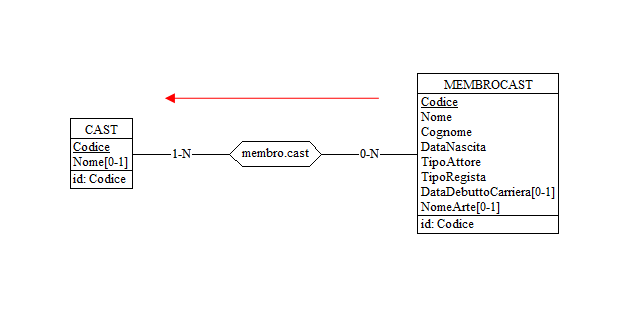
\includegraphics[width=450pt]{ER/navigazione/aggiuntacast.png}
	\caption{Schema di navigazione - aggiunta di persone che hanno realizzato un film}
\end{figure}
\begin{table}[H]
	\centering
	\begin{tabular}{|llll|}
		\hline
		\rowcolor[HTML]{CBCEFB}
		Concetto    & Costrutto & Accesso & Tipo                          \\ \hline
		MEMBROCAST  & E         & 1       & S                             \\ \hline
		membro.cast & R         & 1       & S                             \\ \hline
		\rowcolor[HTML]{CBCEFB}
		\multicolumn{4}{|l|}{\cellcolor[HTML]{FFCE93}\textbf{Totale}: 2S} \\ \hline
	\end{tabular}
\end{table}

\subsubsection{Registrazione di una nuova tessera (Op. 12)}
\begin{figure}[H]
	\centering
	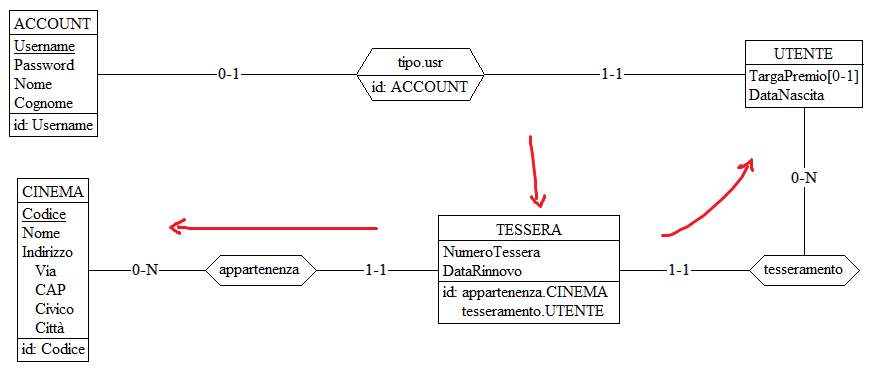
\includegraphics[width=450pt]{ER/navigazione/regtessera.png}
	\caption{Schema di navigazione - Registrazione di una tessera}
\end{figure}
\begin{table}[H]
	\centering
	\begin{tabular}{|llll|}
		\hline
		\rowcolor[HTML]{CBCEFB}
		Concetto     & Costrutto & Accesso & Tipo                         \\ \hline
		TESSERA      & E         & 1       & S                            \\ \hline
		appartenenza & R         & 1       & S                            \\ \hline
		tesseramento & R         & 1       & S                            \\ \hline
		\rowcolor[HTML]{CBCEFB}
		\multicolumn{4}{|l|}{\cellcolor[HTML]{FFCE93}\textbf{Totale}: 3S} \\ \hline
	\end{tabular}
\end{table}


\section{Analisi delle ridondanze}
Le ridondanze principali che vogliamo analizzare sono le seguenti:
\begin{enumerate}
	\item Attributo "NumeroVisualizzati" nell'entità GENERE.
	\item Attributo "DurataComplessiva" nell'entità SERIE.
	\item Attributo "NumeroEpisodi" nell'entità STAGIONE.
	\item Attribito "NumeroStagioni" nell'entità SERIE.
	\item Attributo "VotoComplessivo" nell'entità RECENSIONE.
\end{enumerate}
\subsection{Attributo 1: NumeroVisualizzati}
\subsubsection{Operazioni interessate:}
\begin{itemize}
	\item Op. 8.1: Ottenere una classifica dei generi più visualizzati
	\item Op. 5.(1-2): Contrassegnare come "visualizzato" un film o un episodio di una serie.
\end{itemize}
\subsubsection{Tabelle degli accessi senza ridondanza:}
\begin{itemize}
	\item Per operazione 8.1: Vedi la sottosezione \ref{ss:op81}, essa ha frequenza $5/gg$ dandoci complessivamente 12.743.880 accessi in lettura al giorno.
	\item Per operazione 5.1: Vedi la sottosezione \ref{ss:op51}, essa ha frequenza $350/gg$ dandoci complessivamente 350 accessi in scrittura al giorno.
	\item Per operazione 5.2: Vedi la sottosezione \ref{ss:op52}, essa ha frequenza $500/gg$ dandoci complessivamente 500 accessi in scrittura al giorno.
\end{itemize}
Complessivamente quindi, abbiamo $2 * (500 + 350) + 12.743.880 = 12.745.580$ accessi complessivi.
\subsubsection{Tabelle degli accessi con ridondanza:}
Consideriamo il caso in cui si introduca un attributo ridondante "NumeroVisualizzazioni" sull'entità "GENERE", che viene incrementato ogni volta che un utente contrassegna come visualizzato un film, o tutti gli episodi correnti di una serie.
\begin{itemize}
	\item Per operazione 5.1: Per effettuare questa operazione, oltre che 1S per scrivere la relazione \textit{visualizzazionefilm} è necessario un aggiornamento su genere per incrementare il valore dell'attributo ridondante, avendo una complessità complessiva di 1L + 2S, considerando la frequenza di $350/gg$ questa ci crea $350 + 4 * 350 = 1750$ accessi complessivi al giorno.
	\item Per operazione 5.2: Questa invece ci obbliga a calcolare quanti episodi servono per poter considerare una serie come visualizzata, sappiamo che una serie è composta in media da 4 stagioni da 10 episodi ciascuna, quindi se vengono contrassegnati 500 episodi al giorno, significa che vengono visualizzate in media $\frac{500}{4 * 10} = 12,5$ serie al giorno, comportando 12,5S + 12,5L + 500S accessi, dando una complessità complessiva di $3 * 12,5 + 1000 = 1037,5$ al giorno.
	\item Per operazione 8.1: Con l'attributo ridondante questa operazione si limita alla lettura dell'attributo "NumeroVisualizzati" nell'entità "GENERE", considerando che ce ne sono 13 si hanno 13L con una frequenza di 5 al giorno, quindi complessivamente $13 * 5$ letture al giorno dando una complessità di 65 accessi.
\end{itemize}
In totale si ottiene da questo studio $65 + 1037,5 + 1750 = 2852.5$ accessi complessivi.
\subsubsection{Conclusione:}
Considerando i valori ottenuti dall'analisi precedente, si può affermare che data la complessità $2852.5 \ll 12.745.580$ è di gran lunga conveniente introdurre l'attributo ridondante "NumeroVisualizzati" in GENERE, privilegiando l'efficienza rispetto all'occupazione di spazio.

\subsection{Attributo 2: DurataComplessiva}
\subsubsection{Operazioni interessate:}
\begin{itemize}
	\item Op. 4.3: Visualizzare l’elenco delle serie TV con la relativa durata complessiva e il numero di stagioni ed episodi complessivo, in base all’età di chi lo richiede.
	\item Op. 4.4: Visualizzare le informazioni riguardanti una serie TV, comprese tutte le stagioni e tutti gli episodi.
	\item Op. 4.5: Aggiunta di una nuova stagione per una specifica serie TV.
	\item Op. 4.6: Aggiunta di un nuovo episodio per una specifica stagione di una serie TV.
\end{itemize}
\subsubsection{Tabelle degli accessi senza ridondanza:}
\begin{itemize}
	\item Per operazione 4.3: Vedi la sottosezione \ref{ss:op43}, essa ha frequenza $100/gg$ dandoci complessivamente accessi 41.250.100 in lettura al giorno.
	\item Per operazione 4.4: Vedi la sottosezione \ref{ss:op44}, essa ha frequenza $50/gg$ dandoci complessivamente accessi 2.250 in lettura al giorno.
	\item Per operazione 4.5: Vedi la sottosezione \ref{ss:op45}, essa ha frequenza $5/gg$ dandoci complessivamente accessi 5 in lettura e 40 in scrittura al giorno.
	\item Per operazione 4.6: Vedi la sottosezione \ref{ss:op46}, essa ha frequenza $10/gg$ dandoci complessivamente accessi 10 in lettura e 40 in scrittura al giorno.
\end{itemize}
Complessivamente quindi, abbiamo $41.250.100 + 2.250 + 45 + 50 = 41.252.445$ accessi complessivi.
\subsubsection{Tabelle degli accessi con ridondanza:}
Consideriamo il caso in cui si introduca il seguente attributo ridondante "DurataComplessiva" sull'entità "SERIE", questo attributo serve per dichiarare la durata complessiva(quindi la sommatoria della durata di ciascun episodio) di una serie tv.
\begin{itemize}
	\item Per operazione 4.3: Quest'operazione è analoga al caso senza ridondanza.
	\item Per operazione 4.4: Quest'operazione è analoga al caso senza ridondanza.
	\item Per operazione 4.5: Per questa operazione gli accessi in scrittura aumentano dato che bisogna fare un aggiornamento nell'entità SERIE per incrementare l'attributo ridondante "DurataComplessiva" a seguito dell'aggiunta in STAGIONE ed EPISODIO. Quindi avremo un totale di 1L + 5S che messe in relazione con la frequenza giornaliera darà come risultato un totale di 5 accessi in lettura e 50 accessi in scrittura al giorno.
	\item Per operazione 4.6: Anche in quest'operazione bisogna aumentare la durata complessiva nell'entità SERIE quindi effettuare un aggiornamento ottenendo in totale 2L + 3S che messe in relazione con la frequenza giornaliera darà come risultato un totale di 20 accessi in lettura e 60 accessi in scrittura al giorno.
\end{itemize}

In totale si ottiene da questo studio $41.250.100 + 2.250 + 55 + 80 = 41.252.485$ accessi complessivi.
\subsubsection{Conclusioni:}
Considerando i valori ottenuti dall'analisi precedente, possiamo affermare che data la complessità $41.252.485 > 41.252.445$ NON conviene introdurre l'attributo ridondante "DurataComplessiva" in SERIE (perlomeno non singolarmente).

\subsection{Attributo 3: NumeroEpisodi}
\subsubsection{Operazioni interessate:}
\begin{itemize}
	\item Op. 4.3: Visualizzare l’elenco delle serie TV con la relativa durata complessiva e il numero di stagioni ed episodi complessivo, in base all’età di chi lo richiede.
	\item Op. 4.4: Visualizzare le informazioni riguardanti una serie TV, comprese tutte le stagioni e tutti gli episodi.
	\item Op. 4.5: Aggiunta di una nuova stagione per una specifica serie TV.
	\item Op. 4.6: Aggiunta di un nuovo episodio per una specifica stagione di una serie TV.
\end{itemize}
\subsubsection{Tabelle degli accessi senza ridondanza:}
\begin{itemize}
	\item Per operazione 4.3: Vedi la sottosezione \ref{ss:op43}, essa ha frequenza $100/gg$ dandoci complessivamente accessi 41.250.100 in lettura al giorno.
	\item Per operazione 4.4: Vedi la sottosezione \ref{ss:op44}, essa ha frequenza $50/gg$ dandoci complessivamente accessi 2.250 in lettura al giorno.
	\item Per operazione 4.5: Vedi la sottosezione \ref{ss:op45}, essa ha frequenza $5/gg$ dandoci complessivamente accessi 5 in lettura e 40 in scrittura al giorno.
	\item Per operazione 4.6: Vedi la sottosezione \ref{ss:op46}, essa ha frequenza $10/gg$ dandoci complessivamente accessi 10 in lettura e 40 in scrittura al giorno.
\end{itemize}
Complessivamente quindi, abbiamo $41.250.100 + 2.250 + 45 + 50 = 41.252.445$ accessi complessivi.
\subsubsection{Tabelle degli accessi con ridondanza:}
Consideriamo il caso in cui si introduca il seguente attributo ridondante "NumeroEpisodi" sull'entità "STAGIONE", questo attributo serve per dichiarare la quantità di episodi che è composta una STAGIONE di una specifica SERIE.
\begin{itemize}
	\item Per operazione 4.3: Quest'operazione è analoga al caso senza ridondanza.
	\item Per operazione 4.4: Quest'operazione è analoga al caso senza ridondanza.
	\item Per operazione 4.5: Quest'operazione è analoga al caso senza ridondanza.
	\item Per operazione 4.6: In quest'operazione bisogna incrementare "NumeroEpisodi" nell'entità STAGIONE quindi effettuare un aggiornamento ottenendo in totale 1L + 3S che messe in relazione con la frequenza giornaliera darà come risultato un totale di 10 accessi in lettura e 60 accessi in scrittura al giorno.
\end{itemize}

In totale si ottiene da questo studio $41.250.100 + 2.250 + 45 + 70 = 41.252.465$ accessi complessivi.
\subsubsection{Conclusioni:}
Considerando i valori ottenuti dall'analisi precedente, possiamo affermare che data la complessità $41.252.465 > 41.252.445$ NON conviene introdurre l'attributo ridondante "NumeroEpisodi" in STAGIONE (perlomeno non singolarmente).


\subsection{Attributo 4: NumeroStagioni}
\subsubsection{Operazioni interessate:}
\begin{itemize}
	\item Op. 4.3: Visualizzare l’elenco delle serie TV con la relativa durata complessiva e il numero di stagioni ed episodi complessivo, in base all’età di chi lo richiede.
	\item Op. 4.4: Visualizzare le informazioni riguardanti una serie TV, comprese tutte le stagioni e tutti gli episodi.
	\item Op. 4.5: Aggiunta di una nuova stagione per una specifica serie TV.
	\item Op. 4.6: Aggiunta di un nuovo episodio per una specifica stagione di una serie TV.
\end{itemize}
\subsubsection{Tabelle degli accessi senza ridondanza:}
\begin{itemize}
	\item Per operazione 4.3: Vedi la sottosezione \ref{ss:op43}, essa ha frequenza $100/gg$ dandoci complessivamente accessi 41.250.100 in lettura al giorno.
	\item Per operazione 4.4: Vedi la sottosezione \ref{ss:op44}, essa ha frequenza $50/gg$ dandoci complessivamente accessi 2.250 in lettura al giorno.
	\item Per operazione 4.5: Vedi la sottosezione \ref{ss:op45}, essa ha frequenza $5/gg$ dandoci complessivamente accessi 5 in lettura e 40 in scrittura al giorno.
	\item Per operazione 4.6: Vedi la sottosezione \ref{ss:op46}, essa ha frequenza $10/gg$ dandoci complessivamente accessi 10 in lettura e 40 in scrittura al giorno.
\end{itemize}
Complessivamente quindi, abbiamo $ 41.250.100 + 2.250 + 45 + 50 = 41.252.445$ accessi complessivi.
\subsubsection{Tabelle degli accessi con ridondanza:}
Consideriamo il caso in cui si introduca il seguente attributo ridondante "NumeroStagioni" sull'entità "SERIE", questo attributo serve per dichiarare la quantità di stagioni che è composta una SERIE.
\begin{itemize}
	\item Per operazione 4.3: Quest'operazione è analoga al caso senza ridondanza.
	\item Per operazione 4.4: Quest'operazione è analoga al caso senza ridondanza.
	\item Per operazione 4.5: Per questa operazione è necessario l'incremento dell'attributo ridondante in SERIE, quindi questo aggiornamento porta ad avere gli accessi totali a 1L in lettura e 5S. Mettendo questi accessi in relazione con la frequenza, otteniamo in totale 5 accessi in lettura e 100 accessi in scrittura al giorno.
	\item Per operazione 4.6: Quest'operazione è analoga al caso senza ridondanza.
\end{itemize}

In totale si ottiene da questo studio $41.250.100 + 2.250 + 105 + 50 = 41.252.505$ accessi complessivi.
\subsubsection{Conclusioni:}
Considerando i valori ottenuti dall'analisi precedente, possiamo affermare che data la complessità $41.252.505 > 41.252.445$ NON conviene introdurre l'attributo ridondante "NumeroStagioni" in SERIE (perlomeno non singolarmente).


\subsection{Attributo 2-3: DurataComplessiva e NumeroEpisodi}
\subsubsection{Operazioni interessate:}
\begin{itemize}
	\item Op. 4.3: Visualizzare l’elenco delle serie TV con la relativa durata complessiva e il numero di stagioni ed episodi complessivo, in base all’età di chi lo richiede.
	\item Op. 4.4: Visualizzare le informazioni riguardanti una serie TV, comprese tutte le stagioni e tutti gli episodi.
	\item Op. 4.5: Aggiunta di una nuova stagione per una specifica serie TV.
	\item Op. 4.6: Aggiunta di un nuovo episodio per una specifica stagione di una serie TV.
\end{itemize}
\subsubsection{Tabelle degli accessi senza ridondanza:}
\begin{itemize}
	\item Per operazione 4.3: Vedi la sottosezione \ref{ss:op43}, essa ha frequenza $100/gg$ dandoci complessivamente accessi 41.250.100 in lettura al giorno.
	\item Per operazione 4.4: Vedi la sottosezione \ref{ss:op44}, essa ha frequenza $50/gg$ dandoci complessivamente accessi 2.250 in lettura al giorno.
	\item Per operazione 4.5: Vedi la sottosezione \ref{ss:op45}, essa ha frequenza $5/gg$ dandoci complessivamente accessi 5 in lettura e 40 in scrittura al giorno.
	\item Per operazione 4.6: Vedi la sottosezione \ref{ss:op46}, essa ha frequenza $10/gg$ dandoci complessivamente accessi 10 in lettura e 40 in scrittura al giorno.
\end{itemize}
Complessivamente quindi, abbiamo $41.250.100 + 2.250 + 45 + 50 = 41.252.445$ accessi complessivi.
\subsubsection{Tabelle degli accessi con ridondanza:}
Consideriamo il caso in cui si introducano i seguenti attributi ridondanti "DurataComplessiva" e "NumeroEpisodi" relativamente sulle entità "SERIE" e "STAGIONE", questi attributi servono per sapere la durata totale(in minuti) di una serie e il numero di episodi per una stagione di una serie TV.
\begin{itemize}
	\item Per operazione 4.3: Quest'operazione è analoga al caso senza ridondanza se non per il fatto che non è più necessario leggere ciascun episodio, grazie al fatto che manteniamo salvato il numero di episodi tramite l'attributo ridondante in STAGIONE. Quindi avremo in totale 12.501L, che messe in relazione con la frequenza diventano 1.250.100 accessi in lettura al giorno.
	\item Per operazione 4.4: Quest'operazione è analoga al caso senza ridondanza.
	\item Per operazione 4.5: Per questa operazione gli accessi in scrittura aumentano dato che bisogna fare un aggiornamento nell'entità SERIE per incrementare l'attributo ridondante "DurataComplessiva" ed anche nell'entità STAGIONE per incrementare l'attributo ridondante "NumeroEpisodi" a seguito dell'aggiunta di una STAGIONE con il relativo EPISODIO (aggiunto obbligatoriamente, data la cardinalità). 
	Quindi avremo un totale di 2L + 5S che messe in relazione con la frequenza giornaliera darà come risultato un totale di 10 accessi in lettura e 50 accessi in scrittura al giorno.
	\item Per operazione 4.6: Per questa operazione il ragionamento è analogo alla precedente. Quindi otterremo un totale di 2L + 3S che messe in relazione con la frequenza giornaliera darà come risultato un totale di 20 accessi in lettura e 60 accessi in scrittura al giorno.
\end{itemize}

In totale si ottiene da questo studio $1.250.100 + 2.250 + 60 + 80 = 1.252.490$ accessi complessivi.
\subsubsection{Conclusioni:}
Considerando i valori ottenuti dall'analisi precedente, possiamo affermare che data la complessità $1.252.490 \ll 41.252.445$ conviene introdurre, in coppia, gli attributi ridondanti "DurataComplessiva" e "NumeroEpisodi" relativamente nelle entità SERIE e STAGIONE.


\subsection{Attributo 2-4: DurataComplessiva e NumeroStagioni}
\subsubsection{Operazioni interessate:}
\begin{itemize}
	\item Op. 4.3: Visualizzare l’elenco delle serie TV con la relativa durata complessiva e il numero di stagioni ed episodi complessivo, in base all’età di chi lo richiede.
	\item Op. 4.4: Visualizzare le informazioni riguardanti una serie TV, comprese tutte le stagioni e tutti gli episodi.
	\item Op. 4.5: Aggiunta di una nuova stagione per una specifica serie TV.
	\item Op. 4.6: Aggiunta di un nuovo episodio per una specifica stagione di una serie TV.
\end{itemize}
\subsubsection{Tabelle degli accessi senza ridondanza:}
\begin{itemize}
	\item Per operazione 4.3: Vedi la sottosezione \ref{ss:op43}, essa ha frequenza $100/gg$ dandoci complessivamente accessi 41.250.100 in lettura al giorno.
	\item Per operazione 4.4: Vedi la sottosezione \ref{ss:op44}, essa ha frequenza $50/gg$ dandoci complessivamente accessi 2.250 in lettura al giorno.
	\item Per operazione 4.5: Vedi la sottosezione \ref{ss:op45}, essa ha frequenza $5/gg$ dandoci complessivamente accessi 5 in lettura e 40 in scrittura al giorno.
	\item Per operazione 4.6: Vedi la sottosezione \ref{ss:op46}, essa ha frequenza $10/gg$ dandoci complessivamente accessi 10 in lettura e 40 in scrittura al giorno.
\end{itemize}
Complessivamente quindi, abbiamo $41.250.100 + 2.250 + 45 + 50 = 41.252.445$ accessi complessivi.
\subsubsection{Tabelle degli accessi con ridondanza:}
Consideriamo il caso in cui si introducano i seguenti attributi ridondanti "DurataComplessiva" e "NumeroStagioni" relativamente sulla entità "SERIE", questi attributi servono per sapere la durata totale(in minuti) di una serie e il numero di stagioni per una una serie TV.
\begin{itemize}
	\item Per operazione 4.3: Quest'operazione è analoga al caso senza ridondanza se non per il fatto che non è più necessario leggere ciascuna stagione, grazie al fatto che manteniamo salvato il numero di stagioni tramite l'attributo ridondante in SERIE. Quindi avremo in totale 402.501L, che messe in relazione con la frequenza diventano 40.250.100 accessi in lettura al giorno.
	\item Per operazione 4.4: Quest'operazione è analoga al caso senza ridondanza.
	\item Per operazione 4.5: Per questa operazione gli accessi in scrittura aumentano dato che bisogna fare un aggiornamento nell'entità SERIE per incrementare l'attributo ridondante "DurataComplessiva" e "NumeroStagioni" a seguito dell'aggiunta di una STAGIONE con il relativo EPISODIO (aggiunto obbligatoriamente, data la cardinalità). 
	Quindi avremo un totale di 1L + 5S che messe in relazione con la frequenza giornaliera darà come risultato un totale di 5 accessi in lettura e 50 accessi in scrittura al giorno.
	\item Per operazione 4.6: Per questa operazione il ragionamento è analogo alla precedente. Quindi otterremo un totale di 2L + 3S, aggiornando "DurataComplessiva" di SERIE, che messe in relazione con la frequenza giornaliera darà come risultato un totale di 20 accessi in lettura e 60 accessi in scrittura al giorno.
\end{itemize}

In totale si ottiene da questo studio $40.250.100 + 2.250 + 55 + 80 = 40.252.485$ accessi complessivi.
\subsubsection{Conclusioni:}
Considerando i valori ottenuti dall'analisi precedente, possiamo affermare che data la complessità $40.252.485 < 41.252.445$ conviene introdurre, in coppia, gli attributi ridondanti "DurataComplessiva" e "NumeroStagioni" relativamente nella entità SERIE.


\subsection{Attributo 3-4: NumeroEpisodi e NumeroStagioni}
\subsubsection{Operazioni interessate:}
\begin{itemize}
	\item Op. 4.3: Visualizzare l’elenco delle serie TV con la relativa durata complessiva e il numero di stagioni ed episodi complessivo, in base all’età di chi lo richiede.
	\item Op. 4.4: Visualizzare le informazioni riguardanti una serie TV, comprese tutte le stagioni e tutti gli episodi.
	\item Op. 4.5: Aggiunta di una nuova stagione per una specifica serie TV.
	\item Op. 4.6: Aggiunta di un nuovo episodio per una specifica stagione di una serie TV.
\end{itemize}
\subsubsection{Tabelle degli accessi senza ridondanza:}
\begin{itemize}
	\item Per operazione 4.3: Vedi la sottosezione \ref{ss:op43}, essa ha frequenza $100/gg$ dandoci complessivamente accessi 41.250.100 in lettura al giorno.
	\item Per operazione 4.4: Vedi la sottosezione \ref{ss:op44}, essa ha frequenza $50/gg$ dandoci complessivamente accessi 2.250 in lettura al giorno.
	\item Per operazione 4.5: Vedi la sottosezione \ref{ss:op45}, essa ha frequenza $5/gg$ dandoci complessivamente accessi 5 in lettura e 40 in scrittura al giorno.
	\item Per operazione 4.6: Vedi la sottosezione \ref{ss:op46}, essa ha frequenza $10/gg$ dandoci complessivamente accessi 10 in lettura e 40 in scrittura al giorno.
\end{itemize}
Complessivamente quindi, abbiamo $41.250.100 + 2.250 + 45 + 50 = 41.252.445$ accessi complessivi.
\subsubsection{Tabelle degli accessi con ridondanza:}
Consideriamo il caso in cui si introducano i seguenti attributi ridondanti "NumeroEpisodi" e "NumeroStagioni" relativamente sulle entità "STAGIONE" e "SERIE", questi attributi servono per sapere il numero di episodi di una serie e il numero di stagioni per una serie TV.
\begin{itemize}
	\item Per operazione 4.3: Quest'operazione è analoga al caso senza ridondanza.
	\item Per operazione 4.4: Quest'operazione è analoga al caso senza ridondanza.
	\item Per operazione 4.5: Per questa operazione gli accessi in scrittura aumentano dato che bisogna fare un aggiornamento nell'entità SERIE per incrementare l'attributo ridondante "NumeroStagioni" a seguito dell'aggiunta di un'entità STAGIONE con il relativo EPISODIO (aggiunto obbligatoriamente, data la cardinalità). 
	Quindi avremo un totale di 1L + 5S che messe in relazione con la frequenza giornaliera darà come risultato un totale di 5 accessi in lettura e 50 accessi in scrittura al giorno.
	\item Per operazione 4.6: Per questa operazione il ragionamento è analogo alla precedente. Quindi otterremo un totale di 1L + 3S, che messe in relazione con la frequenza giornaliera darà come risultato un totale di 10 accessi in lettura e 60 accessi in scrittura al giorno.
\end{itemize}

In totale si ottiene da questo studio $41.250.100 + 2.250 + 55 + 70 = 41.252.475$ accessi complessivi.
\subsubsection{Conclusioni:}
Considerando i valori ottenuti dall'analisi precedente, possiamo affermare che data la complessità $41.252.475 > 41.252.445$ NON conviene introdurre, in coppia, gli attributi ridondanti "NumeroEpisodi" e "NumeroStagioni" relativamente nelle entità SERIE e STAGIONE.


\subsection{Attributo 2-3-4: DurataComplessiva, NumeroEpisodi e NumeroStagioni}
\subsubsection{Operazioni interessate:}
\begin{itemize}
	\item Op. 4.3: Visualizzare l’elenco delle serie TV con la relativa durata complessiva e il numero di stagioni ed episodi complessivo, in base all’età di chi lo richiede.
	\item Op. 4.4: Visualizzare le informazioni riguardanti una serie TV, comprese tutte le stagioni e tutti gli episodi.
	\item Op. 4.5: Aggiunta di una nuova stagione per una specifica serie TV.
	\item Op. 4.6: Aggiunta di un nuovo episodio per una specifica stagione di una serie TV.
\end{itemize}
\subsubsection{Tabelle degli accessi senza ridondanza:}
\begin{itemize}
	\item Per operazione 4.3: Vedi la sottosezione \ref{ss:op43}, essa ha frequenza $100/gg$ dandoci complessivamente accessi 41.250.100 in lettura al giorno.
	\item Per operazione 4.4: Vedi la sottosezione \ref{ss:op44}, essa ha frequenza $50/gg$ dandoci complessivamente accessi 2.250 in lettura al giorno.
	\item Per operazione 4.5: Vedi la sottosezione \ref{ss:op45}, essa ha frequenza $5/gg$ dandoci complessivamente accessi 5 in lettura e 40 in scrittura al giorno.
	\item Per operazione 4.6: Vedi la sottosezione \ref{ss:op46}, essa ha frequenza $10/gg$ dandoci complessivamente accessi 10 in lettura e 40 in scrittura al giorno.
\end{itemize}
Complessivamente quindi, abbiamo $41.250.100 + 2.250 + 45 + 50 = 41.252.445$ accessi complessivi.
\subsubsection{Tabelle degli accessi con ridondanza:}
Consideriamo il caso in cui si introducano i seguenti attributi ridondanti "DurataComplessiva", "NumeroStagioni" e "NumeroEpisodi" sulle entità "SERIE" e "STAGIONE", questi attributi servono per sapere la durata complessiva di ciascun episodio, il numero di episodi di una serie e il numero di stagioni per una serie TV.
\begin{itemize}
	\item Per operazione 4.3: Quest'operazione viene ridotta notevolmente visto che abbiamo tutte le informazioni necessarie all'interno dell'entità SERIE e STAGIONE. Quindi in totale saranno fatti 12500L che messe in relazione con la frequenza giornaliera darà come risultato un totale di 1.250.000 accessi in lettura al giorno.
	\item Per operazione 4.4: Quest'operazione è analoga al caso senza ridondanza.
	\item Per operazione 4.5: Per questa operazione gli accessi in scrittura aumentano dato che bisogna fare un aggiornamento nell'entità SERIE per incrementare gli attributi ridondante "NumeroStagioni" e "DurataComplessiva" a seguito dell'aggiunta di un'entità STAGIONE con il relativo EPISODIO (aggiunto obbligatoriamente, data la cardinalità). 
	Quindi avremo un totale di 1L + 5S che messe in relazione con la frequenza giornaliera darà come risultato un totale di 5 accessi in lettura e 50 accessi in scrittura al giorno.
	\item Per operazione 4.6: Per questa operazione il ragionamento è analogo alla precedente. Quindi otterremo un totale di 2L + 4S, che messe in relazione con la frequenza giornaliera darà come risultato un totale di 20 accessi in lettura e 80 accessi in scrittura al giorno.
\end{itemize}

In totale si ottiene da questo studio $1.250.000 + 2.250 + 55 + 100 = 1.252.405$ accessi complessivi.
\subsubsection{Conclusioni:}
Considerando i valori ottenuti dall'analisi precedente, possiamo affermare che data la complessità $1.252.405 \ll 41.252.445$ conviene introdurre, in trio, gli attributi ridondanti "DurataComplessiva", "NumeroStagioni" e "NumeroEpisodi" relativamente nelle entità SERIE e STAGIONE.


\subsection{Attributo 5: VotoComplessivo}
\subsubsection{Operazioni interessate:}
\begin{itemize}
	\item Op. 7.1: Visualizzare le recensioni di un film.
	\item Op. 7.4: Visualizzare le recensioni di una serie.
\end{itemize}
\subsubsection{Tabelle degli accessi senza ridondanza:}
\begin{itemize}
	\item Per operazione 7.1: 600L con una frequenza di $250/gg$.
	\item Per operazione 7.4: 600L con una frequenza di $150/gg$.
\end{itemize}
In tutto abbiamo $600 * 250 + 600 * 150 = 252.500$ accessi complessivi.
\subsubsection{Tabelle degli accessi con ridondanza:}
Supponiamo di introdurre un "VotoComplessivo" su ogni singola recensione, le letture non diminuiscono dato che comunque vanno reperiti i dati sulle diverse sezioni per poterle visualizzare:
\begin{itemize}
	\item Op. 7.1: 600L con una frequenza di $250/gg$.
	\item Op. 7.4: 600L con una frequenza di $150/gg$.
	\item Op. 7.5: 1S + 1L + 5L (il ricalcolo del voto complessivo) con una frequenza di $50/gg$
\end{itemize}
\subsubsection{Conclusione:}
Si nota che nel secondo caso gli accessi sono maggiori rispetto al primo, quindi l'introduzione dell'attributo ridondante non è conveniente.

\subsection{Conclusioni finale sull'analisi delle ridondanze}
A seguito delle analisi svolte sugli attributi che causavano ridondanza all'interno dello schema, è stato deciso di mantenere i seguenti attributi:
\begin{itemize}
	\item \textbf{NumeroVisualizzati} nell'entità GENERE.
	\item \textbf{DurataComplessiva} e \textbf{NumeroStagioni} nell'entità SERIE.
	\item \textbf{NumeroEpisodi} nell'entità STAGIONE.
\end{itemize}

\section{Rimozione degli attributi composti}
CINEMA.Indirizzo composto da Via, CAP, Civico e Città viene scomposto usando disaggregazione in Ind{\_}Via, Ind{\_}CAP, Ind{\_}Civico e Ind{\_}Città.
\section{Traduzione di entità e associazioni in relazioni}
\subsection{Schema tradotto}
\begin{figure}[H]
	\centering
	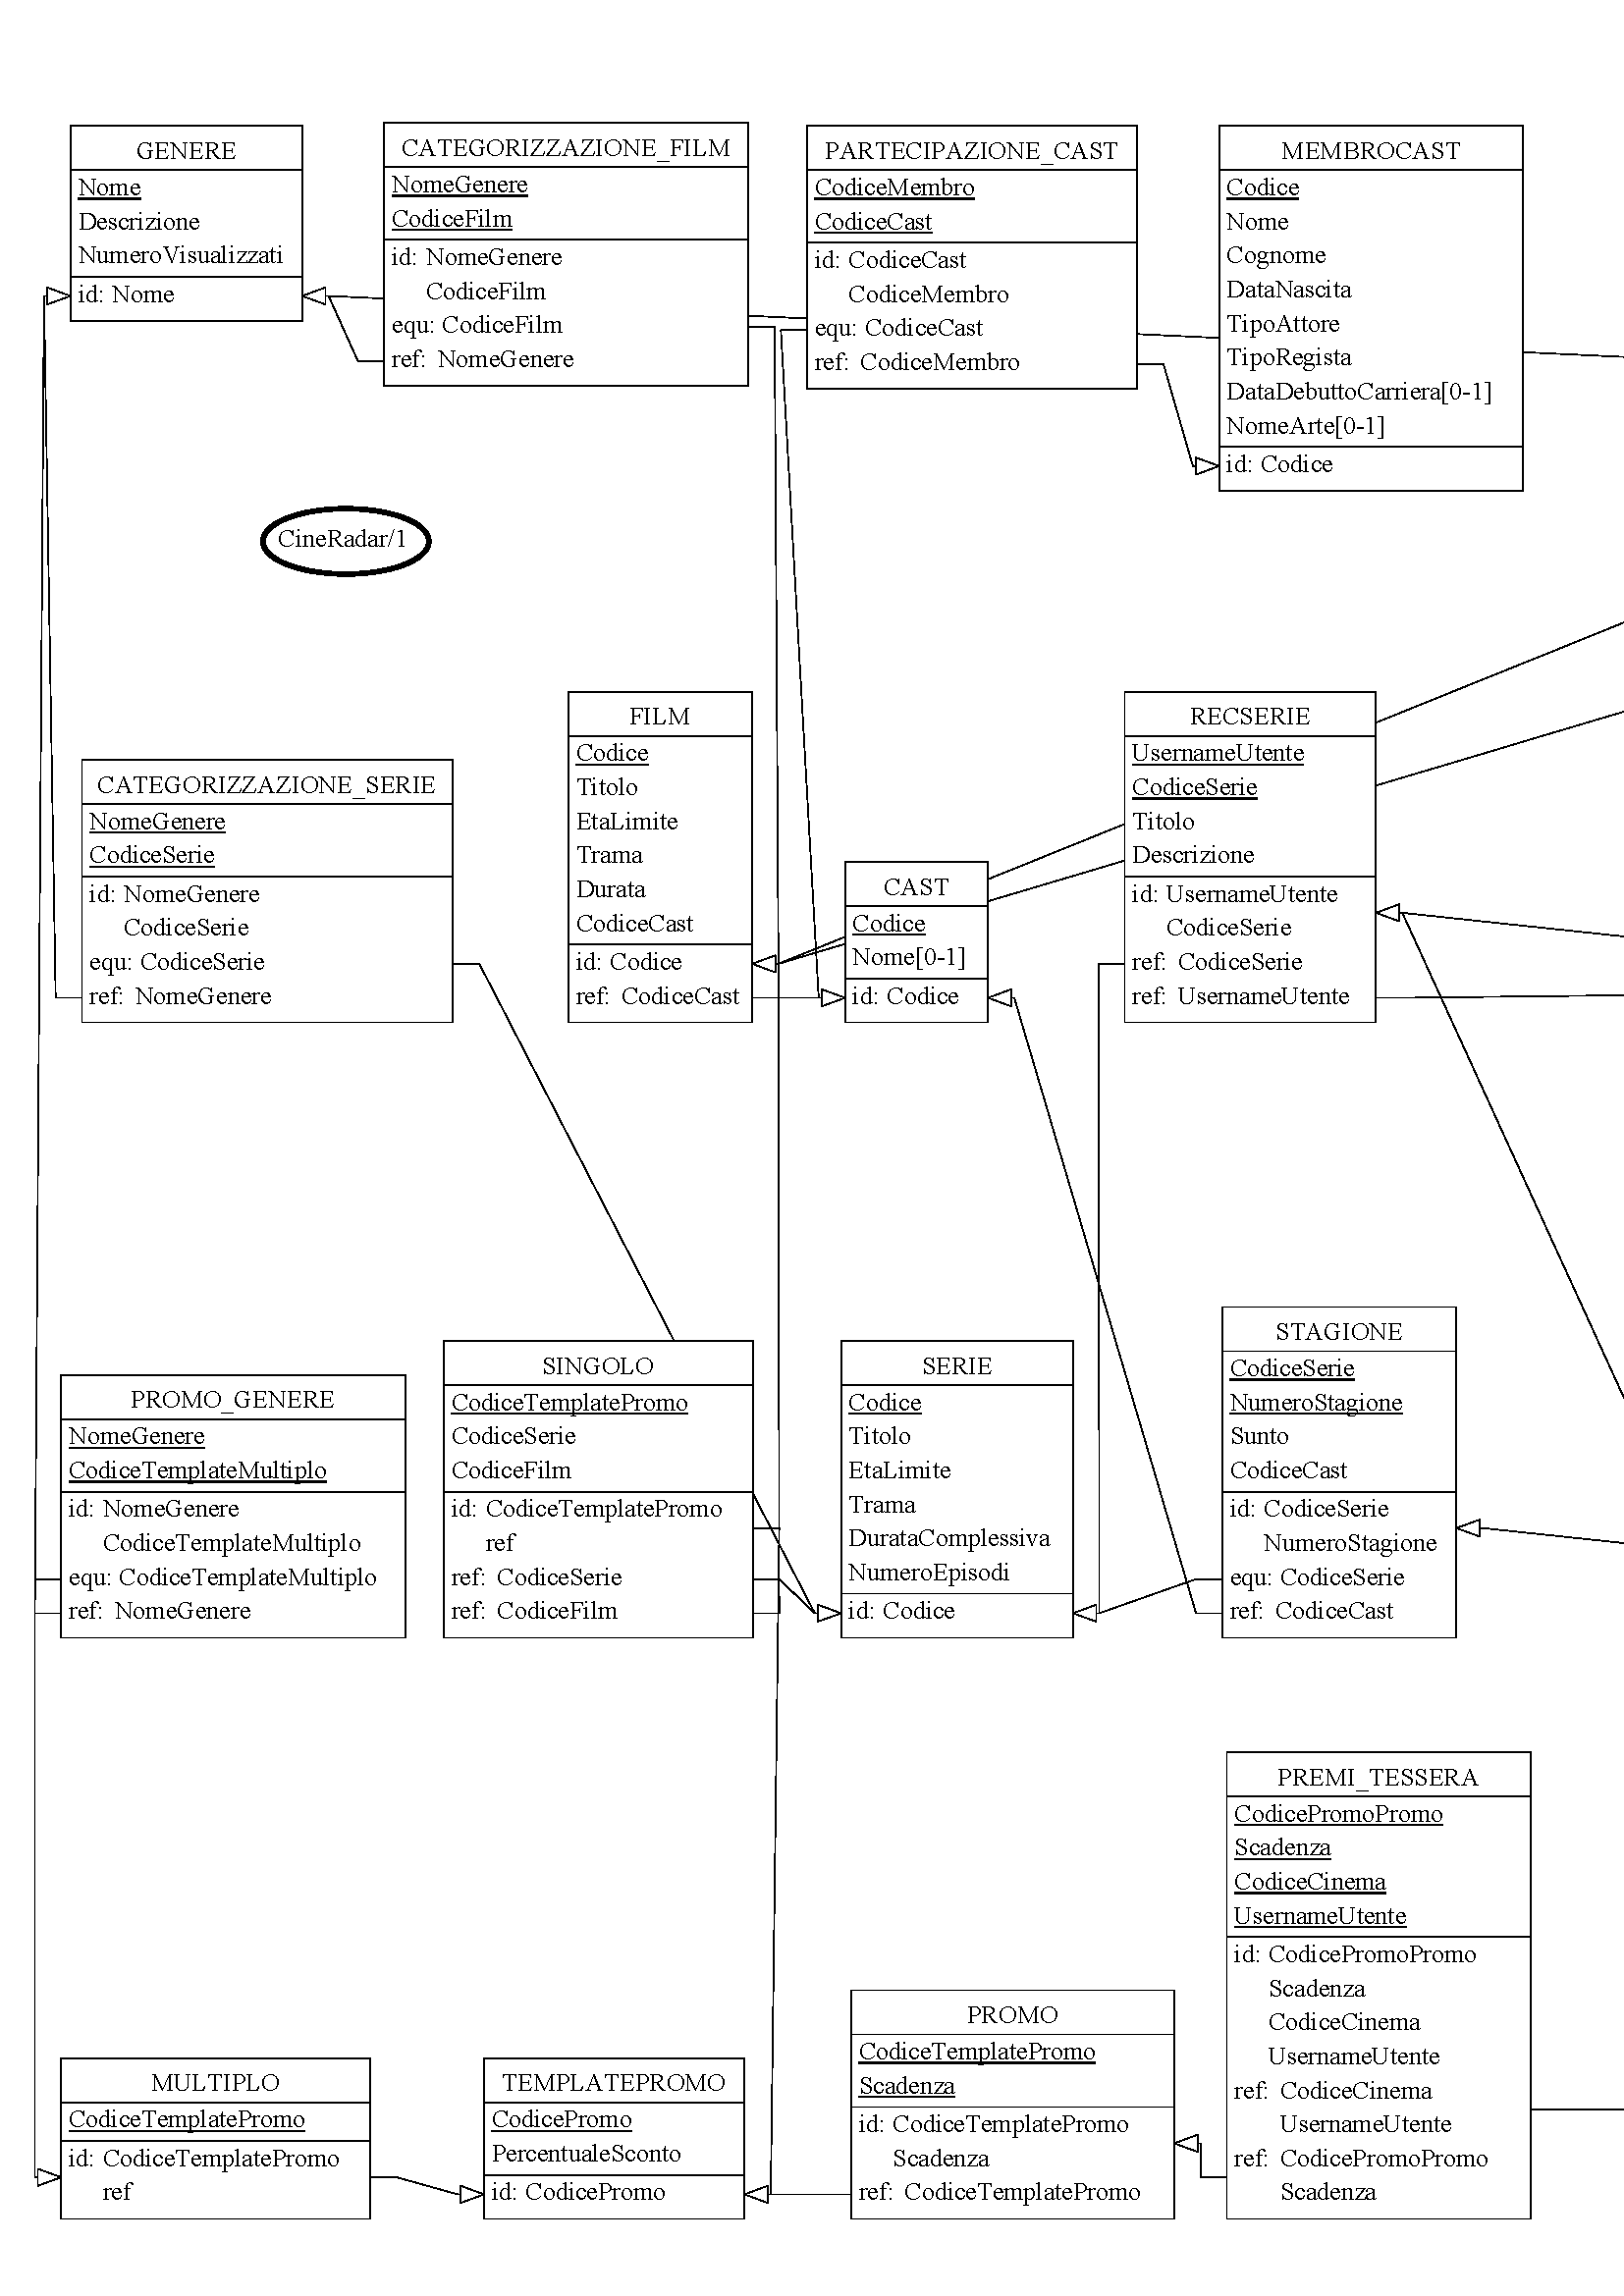
\includegraphics[width=350pt]{ER/schemalogico/logicsx.png}
\end{figure}
\begin{figure}[H]
	\centering
	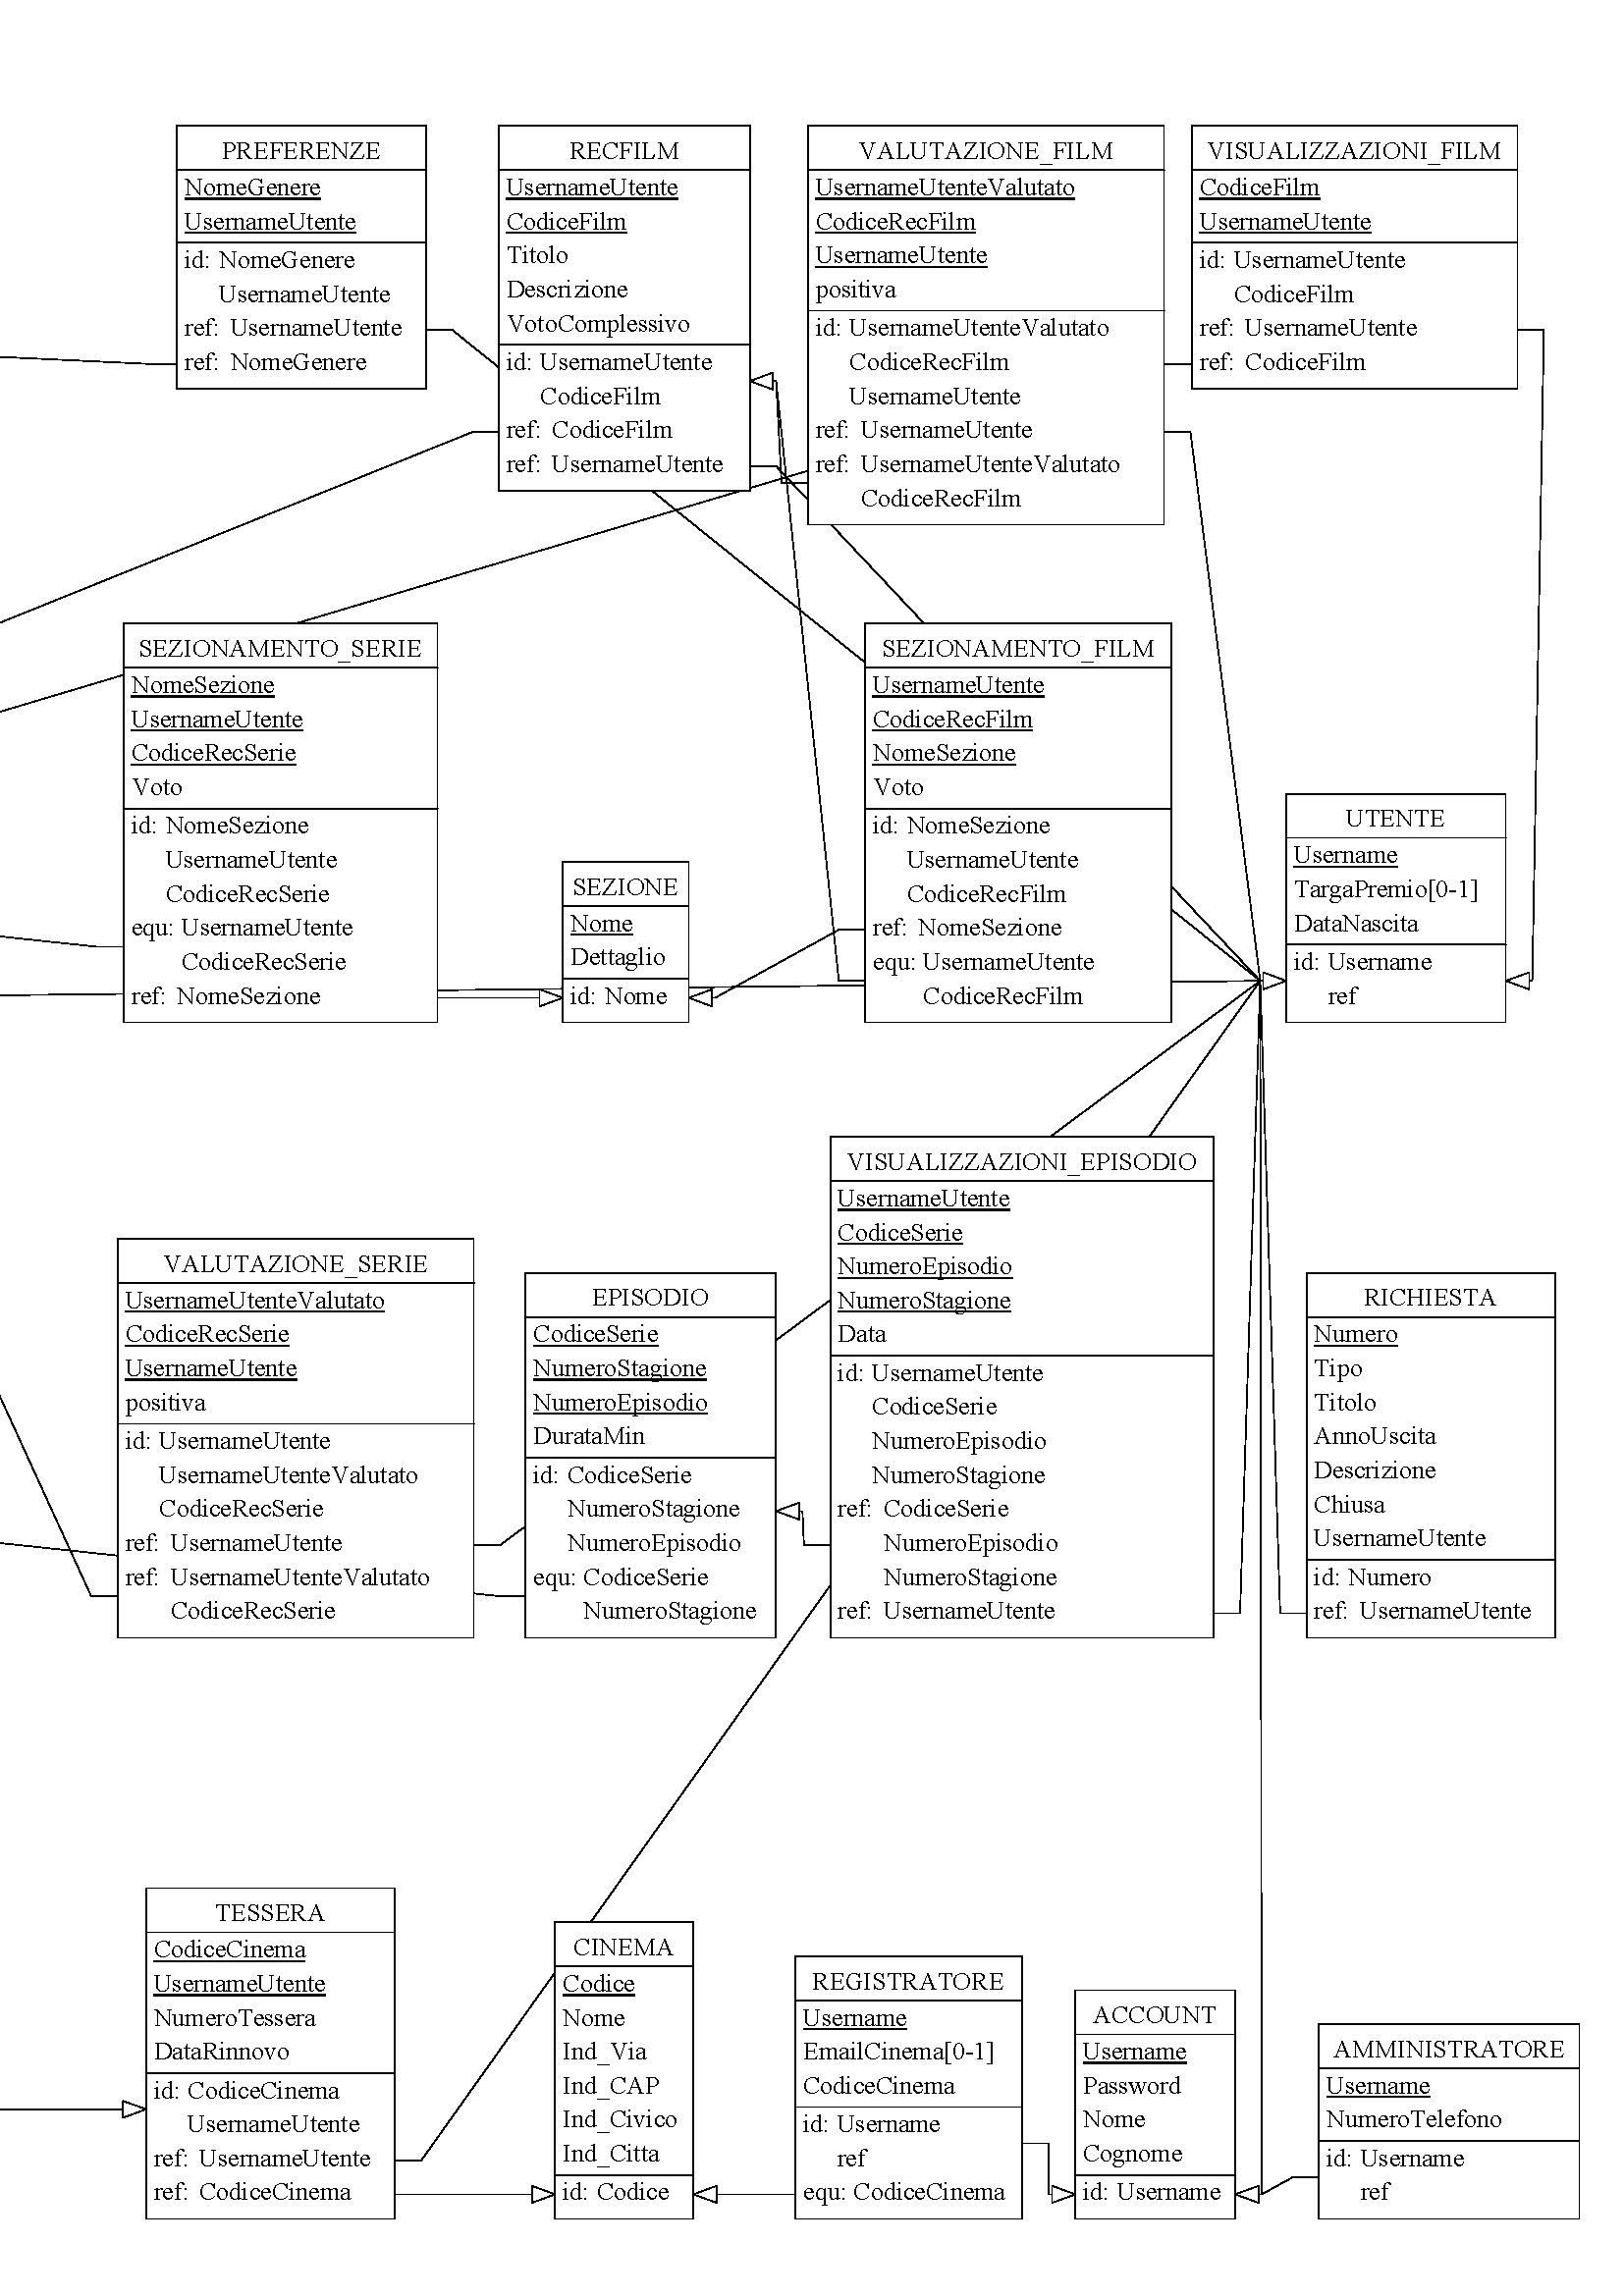
\includegraphics[width=350pt]{ER/schemalogico/logicdx.png}
\end{figure}

\subsection{Schema logico}
\begin{itemize} % Ho lasciato gli spazi per poter suddividere meglio a vista le varie "categorie" di Entità.
	\item \textbf{GENERE}(\underline{Nome}, Descrizione, NumeroVisualizzati)
	
	\item \textbf{CAST}(\underline{Codice}, Nome*)
	
	\item \textbf{FILM}(\underline{Codice}, Titolo, EtaLimite, Trama, Durata, CodiceCast:CAST)
	\item \textbf{CATEGORIZZAZIONE{\_}FILM}(\underline{NomeGenere}:GENERE, \underline{CodiceFilm}:FILM)
	
	\item \textbf{SERIE}(\underline{Codice}, Titolo, EtaLimite, Trama, DurataComplessiva, NumeroEpisodi)
	\item \textbf{STAGIONE}(\underline{CodiceSerie}:SERIE, \underline{NumeroStagione}, Sunto, CodiceCast:CAST)
	\item \textbf{EPISODIO}(\underline{CodiceSerie}:STAGIONE, \underline{NumeroStagione}:STAGIONE, \underline{NumeroEpisodio}, DurataMin)
	\item \textbf{CATEGORIZZAZIONE{\_}SERIE}(\underline{NomeGenere}:GENERE, \underline{CodiceSerie}:SERIE)
	
	\item \textbf{SEZIONE}(\underline{Nome}, Dettaglio)
	
	\item \textbf{TEMPLATEPROMO}(\underline{CodicePromo}, PercentualeSconto)
	\item \textbf{PROMO}(\underline{CodiceTemplatePromo}:TEMPLATEPROMO, \underline{Scadenza})
	\item \textbf{SINGOLO}(\underline{CodiceTemplatePromo}:TEMPLATEPROMO, CodiceSerie:SERIE, CodiceFilm:FILM)
	\item \textbf{MULTIPLO}(\underline{CodiceTemplatePromo}:TEMPLATEPROMO)
	\item \textbf{PROMO{\_}GENERE}(\underline{NomeGenere}:GENERE, \underline{CodiceTemplateMultiplo}:MULTIPLO)
	
	\item \textbf{CINEMA}(\underline{Codice}, Nome, Ind{\_}Via, Ind{\_}CAP, Ind{\_}Civico, Ind{\_}Citta)
	
	\item \textbf{ACCOUNT}(\underline{Username}, Password, Nome, Cognome)
	\item \textbf{UTENTE}(\underline{Username}:ACCOUNT, TargaPremio*, DataNascita)
	\item \textbf{AMMINISTRATORE}(\underline{Username}:ACCOUNT, NumeroTelefono)
	\item \textbf{REGISTRATORE}(\underline{Username}:ACCOUNT, EmailCinema*, CodiceCinema:CINEMA)
	
	\item \textbf{MEMBROCAST}(\underline{Codice}, Nome, Cognome, DataNascita, TipoAttore, TipoRegista, DataDebuttoCarriera*, NomeArte*)
	\item \textbf{PARTECIPAZIONE{\_}CAST}(\underline{CodiceMembro}:MEMBROCAST, \underline{CodiceCast}:CAST)
	
	\item \textbf{PREFERENZA}(\underline{NomeGenere}:GENERE, \underline{UsernameUtente}:UTENTE)
	
	\item \textbf{TESSERA}(\underline{CodiceCinema}:CINEMA, \underline{UsernameUtente}:UTENTE, NumeroTessera, DataRinnovo)
	\item \textbf{PREMI{\_}TESSERA}(\underline{CodicePromo}:PROMO, \underline{Scadenza}:PROMO, \underline{CodiceCinema}:TESSERA, \underline{UsernameUtente}:TESSERA)
	
	\item \textbf{RECSERIE}(\underline{UsernameUtente}:UTENTE, \underline{CodiceSerie}:SERIE, Titolo, Descrizione)
	\item \textbf{SEZIONAMENTO{\_}SERIE}(\underline{NomeSezione}:SEZIONE, \underline{UsernameUtente}:RECSERIE, \underline{CodiceRecSerie}:RECSERIE, Voto)
	\item \textbf{VALUTAZIONE{\_}SERIE}(\underline{UsernameUtenteValutato}:RECSERIE, \underline{CodiceRecSerie}:RECSERIE, \underline{UsernameUtente}:UTENTE, Positiva)
	
	\item \textbf{RECFILM}(\underline{UsernameUtente}:UTENTE, \underline{CodiceFilm}:FILM, Titolo, Descrizione, VotoComplessivo)
	\item \textbf{SEZIONAMENTO{\_}FILM}(\underline{UsernameUtente}:RECFILM, \underline{CodiceRecFilm}:RECFILM, \underline{NomeSezione}:SEZIONE, Voto)
	\item \textbf{VALUTAZIONE{\_}FILM}(\underline{UsernameUtenteValutato}:RECFILM, \underline{CodiceRecFilm}:RECFILM, \underline{UsernameUtente}:UTENTE, Positiva)
	
	\item \textbf{VISUALIZZAZIONI{\_}EPISODIO}(\underline{UsernameUtente}:UTENTE, \underline{CodiceSerie}:EPISODIO, \underline{NumeroEpisodio}:EPISODIO, \underline{NumeroStagione}:EPISODIO, Data)
	\item \textbf{VISUALIZZAZIONI{\_}FILM}(\underline{CodiceFilm}:FILM, \underline{UsernameUtente}:UTENTE)
	
	\item \textbf{RICHIESTA}(\underline{Numero}, Tipo, Titolo, AnnoUscita, Descrizione, Chiusa, UsernameUtente:UTENTE)
\end{itemize}

\section{Vincoli Intra-Relazionali}
\begin{itemize}
	\item GENERI:
	\begin{itemize}
		\item Vincoli di Dominio:
			\begin{itemize}
				\item Nome: stringa (non vuota)
				\item Descrizione: stringa
				\item NumeroVisualizzati: intero non negativo
			\end{itemize}
		\item Vincoli di Tupla: Nessuno
		\item Vincoli di Chiave: Nome
	\end{itemize}
	\item CAST:
	\begin{itemize}
		\item Vincoli di Dominio:
		\begin{itemize}
			\item Codice: stringa (non vuota)
			\item Nome: stringa
		\end{itemize}
		\item Vincoli di Tupla: Nessuno
		\item Vincoli di Chiave: Codice
	\end{itemize}
	\item FILM:
	\begin{itemize}
		\item Vincoli di Dominio:
		\begin{itemize}
			\item Codice: stringa (non vuota)
			\item Titolo: stringa
			\item EtaLimite: intero non negativo
			\item Trama: stringa
			\item Durata: intero positivo
		\end{itemize}
		\item Vincoli di Tupla: Nessuno
		\item Vincoli di Chiave: Codice
	\end{itemize}
	\item CATEGORIZZAZIONE FILM:
	\begin{itemize}
		\item Vincoli di Dominio: Nessuno
		\item Vincoli di Tupla: Nessuno
		\item Vincoli di Chiave: NomeGenere, Codice
	\end{itemize}
	\item SERIE:
	\begin{itemize}
		\item Vincoli di Dominio:
		\begin{itemize}
			\item Codice: stringa (non vuota)
			\item Titolo: stringa
			\item EtaLimite: intero non negativo
			\item Trama: stringa
			\item DurataComplessiva: intero positivo
			\item NumeroEpisodi: intero positivo
		\end{itemize}
		\item Vincoli di Tupla: Nessuno
		\item Vincoli di Chiave: Codice
	\end{itemize}
	\item STAGIONI:
	\begin{itemize}
		\item Vincoli di Dominio:
		\begin{itemize}
			\item NumeroStagione: intero positivo
			\item Sunto: stringa
		\end{itemize}
		\item Vincoli di Tupla: Nessuno
		\item Vincoli di Chiave: CodiceSerie, NumeroStagione
	\end{itemize}
	\item EPISODI:
	\begin{itemize}
		\item Vincoli di Dominio:
		\begin{itemize}
			\item NumeroEpisodio: intero positivo
			\item DurataMin: intero positivo
		\end{itemize}
		\item Vincoli di Tupla: Nessuno
		\item Vincoli di Chiave: CodiceSerie, NumeroStagione, NumeroEpisodio
	\end{itemize}
	\item CATEGORIZZAZIONE SERIE:
	\begin{itemize}
		\item Vincoli di Dominio: Nessuno
		\item Vincoli di Tupla: Nessuno
		\item Vincoli di Chiave: NomeGenere, CodiceSerie
	\end{itemize}
	\item SEZIONI:
	\begin{itemize}
		\item Vincoli di Dominio:
		\begin{itemize}
			\item Nome: stringa (non vuota)
			\item Dettaglio: stringa
		\end{itemize}
		\item Vincoli di Tupla: Nessuno
		\item Vincoli di Chiave: Nome
	\end{itemize}
	\item TEMPLATEPROMO:
	\begin{itemize}
		\item Vincoli di Dominio:
		\begin{itemize}
			\item CodicePromo: stringa (non vuota)
			\item PercentualeSconto: intero compreso tra 0 e 100
		\end{itemize}
		\item Vincoli di Tupla: Nessuno
		\item Vincoli di Chiave: CodicePromo
	\end{itemize}
	\item PROMO:
	\begin{itemize}
		\item Vincoli di Dominio: Nessuno
		\item Vincoli di Tupla: Nessuno
		\item Vincoli di Chiave: CodiceTemplatePromo, Scadenza
	\end{itemize}
	\item SINGOLI:
	\begin{itemize}
		\item Vincoli di Dominio: Nessuno
		\item Vincoli di Tupla: Nessuno
		\item Vincoli di Chiave: CodiceTemplatePromo, CodiceSerie, CodiceFilm
	\end{itemize}
	\item MULTIPLI:
	\begin{itemize}
		\item Vincoli di Dominio:
		\begin{itemize}
			\item CodiceTemplatePromo: stringa (non vuota)
		\end{itemize}
		\item Vincoli di Tupla: Nessuno
		\item Vincoli di Chiave: CodiceTemplatePromo
	\end{itemize}
	\item PROMO GENERE:
	\begin{itemize}
		\item Vincoli di Dominio: Nessuno
		\item Vincoli di Tupla: Nessuno
		\item Vincoli di Chiave: NomeGenere, CodiceTemplateMultiplo
	\end{itemize}
	\item CINEMA:
	\begin{itemize}
		\item Vincoli di Dominio:
		\begin{itemize}
			\item Codice: stringa (non vuota)
			\item Nome: stringa
			\item IndVia: stringa
			\item IndCAP: stringa
			\item IndCivico: stringa
			\item IndCitta: stringa
		\end{itemize}
		\item Vincoli di Tupla: Nessuno
		\item Vincoli di Chiave: Codice
	\end{itemize}
	\item ACCOUNT:
	\begin{itemize}
		\item Vincoli di Dominio:
		\begin{itemize}
			\item Username: stringa (non vuota)
			\item Password: stringa
			\item Nome: stringa
			\item Cognome: stringa
		\end{itemize}
		\item Vincoli di Tupla: Nessuno
		\item Vincoli di Chiave: Username
	\end{itemize}
	\item UTENTI:
	\begin{itemize}
		\item Vincoli di Dominio:
		\begin{itemize}
			\item DataNascita: data
		\end{itemize}
		\item Vincoli di Tupla: Nessuno
		\item Vincoli di Chiave: Username
	\end{itemize}
	\item AMMINISTRATORI:
	\begin{itemize}
		\item Vincoli di Dominio:
		\begin{itemize}
			\item NumeroTelefono: stringa
		\end{itemize}
		\item Vincoli di Tupla: Nessuno
		\item Vincoli di Chiave: Username
	\end{itemize}
	\item REGISTRATORI:
	\begin{itemize}
		\item Vincoli di Dominio:
		\begin{itemize}
			\item EmailCinema: stringa
		\end{itemize}
		\item Vincoli di Tupla: Nessuno
		\item Vincoli di Chiave: Username
	\end{itemize}
	\item MEMBRICAST:
	\begin{itemize}
		\item Vincoli di Dominio:
		\begin{itemize}
			\item DataNascita: data
			\item TipoAttore: stringa
			\item TipoRegista: stringa
		\end{itemize}
		\item Vincoli di Tupla: Nessuno
		\item Vincoli di Chiave: Codice
	\end{itemize}
\end{itemize}
\subsection{Vincoli di Integritá Referenziale}
\todo{TBD}

\section{Schema relazionale finale}
\todo{TBD}
\section{Traduzione delle operazioni in query SQL}
\todo{TBD}
\chapter{Progettazione dell'applicazione}
\todo{TBD}
\end{document}